\documentclass[twoside,numberorder]{csbachelor}

%==============================================================
%==============================================================

\usepackage{url}
\usepackage{subfigure}

% 张海:其他引用
\usepackage[hidelinks]{hyperref}
\setlength{\LTpre}{1em}
\setlength{\LTpost}{1em}

\usepackage{tikz}
\usetikzlibrary{arrows,backgrounds,fit,shapes}
\tikzstyle{layer} = [draw, dashed]
\tikzstyle{block} = [draw, rectangle, minimum height=2em]
\tikzset{>=latex}

% 一些全局工具的定义
\DeclareMathOperator*{\argmin}{arg\,min}
\DeclareMathOperator*{\argmax}{arg\,max}

%==============================================================
%==============================================================

\begin{document}

%==============================================================
%==============================================================

  % 论文题目:{中文}{英文}
  \zjutitle{标题}
           {Title}
  % 作者:{中文姓名}{英文}{学号}
  \zjuauthor{姓名}{Name}{313XXXXXXXX}
  % 指导教师:{导师中文名}{导师英文名}
  \zjumentor{导师姓名}{Supervisor name}
  % 个人信息:{年级}{专业名称}
  \zjuinfo{2013级}{计算机科学与技术}{Computer Science and Technology}
  % 学院信息:{学院中文}{学院英文}
  \zjucollege{计算机科学与技术学院}{College of Computer Science and Technology}
  % 日期:{提交日期}{Submitted Date}
  \zjudate{2017 年 6 月 5 日}{June 5, 2017}

%==============================================================

  {
    \pagestyle{empty}

    {
  \setlength{\parindent}{0em}

  {
    \linespread{1}

    \vspace*{-1em}

    \begin{center}
      
\includegraphics[width=108mm]{images/xiaoming}
    \end{center}

    \vspace{-1.5em}

    {
      \songti\erhao\bfseries
      \centering
      本~~科~~生~~毕~~业~~设~~计 \par
    }

    \vspace{1em}

    \begin{center}
      
\includegraphics[width=35mm]{images/xiaobiao}
    \end{center}
  }

  \vspace{9em}

  {
    \linespread{1.6}
    \songti\sanhao\bfseries
    \centering
    \newlength{\titlelength}
    \setlength{\titlelength}{22em}
    题目 \; \underline{\makebox[\titlelength]{\zjutitlec}} \\
    姓名 \; \underline{\makebox[\titlelength]{\zjuauthornamec}} \\
    学号 \; \underline{\makebox[\titlelength]{\zjuauthorid}} \\
    指导教师 \; \underline{\makebox[\titlelength - 2em]{\zjumentorc}} \\
    合作导师 \; \underline{\makebox[\titlelength - 2em]{赵挺}} \\
    年级与专业 \; \underline{\makebox[\titlelength - 3em]{\zjugrade \; \zjumajorc}} \\
    学院 \; \underline{\makebox[\titlelength]{\zjucollegec}} \\
    提交日期 \; \underline{\makebox[\titlelength - 2em]{\zjudatec}} \par
  }
}

    {
  \setlength{\parindent}{0em}
  \linespread{1}

  \vspace*{-2.3em}

  {
    \songti\xiaoer
    \centering
    A Thesis Submitted to Zhejiang University \\
    for the Degree of Bachelor of Engineering \par
  }

  \vspace{3.6em}

  \begin{center}
    
\includegraphics[width=29.5mm]{images/xiaobiao}
  \end{center}

  \vspace{3em}

  {
    \songti\xiaoer
    \centering
    TITLE \; \underline{\makebox[17em]{\zjutitlee}} \par
    %TITLE \; \begin{minipage}[t]{17em}\ul\zjutitlee\ul{~~~~~~~~~~~~~~~~~~~~~~}\end{minipage}
  }

  \vspace{1.1em}

  {
    \linespread{2}
    \begin{center}
    \sanhao
    \newlength{\majorlength}
    \setlength{\majorlength}{16em}
    \begin{tabular}{l l}
      Author & \underline{\makebox[\majorlength]{\zjuauthornamee}} \\
      Student ID & \underline{\makebox[\majorlength]{\zjuauthorid}} \\
      Supervisor & \underline{\makebox[\majorlength]{\zjumentore}} \\
      Major & \underline{\makebox[\majorlength]{\zjumajore}} \\
      College & \hspace{-3em}\underline{\makebox[\majorlength + 3em]{\zjucollegee}} \\
      Submitted Date & \underline{\makebox[\majorlength]{\zjudatee}} \\
    \end{tabular} \par
    \end{center}
  }
}


    {
  \setlength{\parindent}{0em}
  \linespread{1}

  \vspace*{0.6em}

  {
    \centering
    \songti\xiaoer
    浙江大学本科生毕业论文(设计)独创性声明 \par
  }

  \vspace{3.1em}

  {
    \setlength{\parindent}{2em}
    \linespread{1.6}
    \songti\xiaosi
    本人声明所呈交的毕业论文(设计)是本人在导师指导下进行的研究工作及取得的研究成果。除了文中特别加以标注和致谢的地方外,文中不包含其他人已经发表或撰写过的研究成果,也不包含为获得 \underline{\kaiti\sihao\bfseries \makebox[5em]{浙江大学}} 或其他教育机构的学位或证书而使用过的材料。与我一同工作的同志对本研究所做的任何贡献均已在文中作了明确的说明并表示谢意。 \par
  }

  \vspace{2.9em}

  {
    \songti\xiaosi
    \begin{tabular}{@{} p{0.5\linewidth} p{0.5\linewidth} @{}}
    作者签名: & 日期: \hspace{4em} 年 \hspace{2em} 月 \hspace{2em} 日 \\
    \end{tabular} \par
  }

  \vspace{4.85em}

  {
    \centering
    \songti\xiaoer
    毕业论文(设计)版权使用授权书 \par
  }

  \vspace{2.2em}

  {
    \setlength{\parindent}{2em}
    \linespread{1.6}
    \songti\xiaosi
    本文作者完全了解 \underline{\kaiti\sihao\bfseries \makebox[5em]{浙江大学}} 有权保留并向国家有关部门或机构送交本文的复印件和磁盘,允许本文被查阅和借阅。本人授权 \underline{\kaiti\sihao\bfseries \makebox[5em]{浙江大学}} 可以将毕业论文(设计)的全部或部分内容编入有关数据库进行检索和传播,可以采用影印、缩印或扫描等复制手段保存、汇编毕业论文(设计)。

    (保密的毕业论文(设计)在解密后适用本授权书) \par
  }

  \vspace{2.9em}

  {
    \songti\xiaosi
    \begin{tabular}{@{} p{0.5\linewidth} p{0.5\linewidth} @{}}
    作者签名: & 导师签名: \\
     & \\
     & \\
    日期: \hspace{4em} 年 \hspace{2em} 月 \hspace{2em} 日 & 日期: \hspace{4em} 年 \hspace{2em} 月 \hspace{2em} 日 \\
    \end{tabular} \par
  }
}

    \cleardoublepage
  }

  {
    \frontmatter

    \pagestyle{frontmatter}
    \makeatletter
      \let\ps@plain\ps@frontmatter
    \makeatother

    \chapter{摘要}

根据原始神经元图像信息进行神经元追踪与数字重建是神经科学界热门方向。神经科学家通过神经元追踪与数字重建,可以反推大脑是如何运作的,对理解智慧的产生有重要的帮助。由于神经元拓扑结构的复杂,自动化重建结果的细节仍然需要研究人员进行人工纠正和修改,以确保数字重建工作的准确性,研究人员还需要进行一些诸如添加或删除网络分支的编辑操作。现有的神经元追踪和数字重建软件大多运行在单机上,无法满足多用户协同编辑与修改的需求,不利于结构脑图谱的分享与交流。随着计算机性能和网络速度的提升,在线实时编辑神经网络结构成为了可能。在这样的背景下,设计并实现一个在线多用户的神经元网络结构编辑分享平台,利用互联网便于数据共享与交流的特点,使神经科学家可以便捷地进行异地,多用户协同编辑神经元网络结构,并分享完成重建的结构脑图谱。实验与测试结果表明,该平台足以支撑至少千名用户同时编辑的需求,并能在毫秒级别的时间内做出响应,达到了实时操作的要求,为神经科学家协同编辑神经元结构与分享成果提供了便利。

{
    \vspace{1em}
    \setlength{\parindent}{0em}
    \textbf{关键词} \; 生物图像信息 \; 神经元重建 \; 实时编辑平台 \par
}
    \chapter{Abstract}

Neuron tracing and digital reconstruction from original neural image information is a hot direction of neural science. By the reconstruction of brain connectome, neuroscientists can speculate how the brain works which is helpful to understand the intelligence. Because of the complexity of the topological structure of neurons, and in some details on the results of automation reconstruction researchers still need to manually correct and modify the results of digital reconstruction, in order to ensure the accuracy of the digital reconstruction. In addition, researchers need to edit the result of the digital reconstruction such as add or delete some branches, etc. Existing neurons tracking for original neural image and digital reconstruction softwares are mostly run on stand-alone, unable to meet the requirements of multi-user collaborative editing and modification, but also not conducive to the exchange of brain connectom. Improvements in computer performance and network speed make it possible for online real-time editing of neural network structures. In such a background, We have designed and implemented a neural network structure of online multi-user edit sharing platform, using the Internet which can facilitate data sharing and exchange can easily carry out off-site, edit neural network structure with multi-user cooperation, and share brain connectome. Experiments and test reports show that the platform is sufficient to support the needs of at least thousands of users editing at the same time, response in milliseconds, meets the real-time operation requirements which provides convenience for neurologists in neuronal tracking and digital reconstruction.

{
    \vspace{1em}
    \setlength{\parindent}{0em}
    \textbf{Keywords} \; bioimage informatics \;  neuron tracing \; real-time editing platform \par
}


    \tableofcontents
    \newpage
    \thispagestyle{empty}
  }

  {
    \mainmatter

    \pagestyle{mainmatter}
    \makeatletter
      \let\ps@plain\ps@mainmatter
    \makeatother

    \newcommand{\upcite}[1]{\textsuperscript{\textsuperscript{\cite{#1}}}}
\chapter{绪论}
\section{背景与意义}

根据原始神经元图像信息的神经元追踪和数字重建是神经科学界热门方向。神经元的形态反应出它的功能,相同功能的神经元通常具有类似的功能。神经科学家通过结构脑图谱的重建,可以反推大脑是如何运作,对理解智慧的产生有重要的帮助。十九世纪以来,神经科学家们开始推测记忆,甚至个性与智力都和大脑神经元之间的连接有密切的联系。图 \ref{worm} 展示了秀丽隐杆线虫的神经结构的神经结构,图中每一个节点均代表一个神经元,每一条线代表一个连接。它仅仅由 300 个神经元组成,之间的连接也仅有 7000 个。

\begin{figure}
\centering
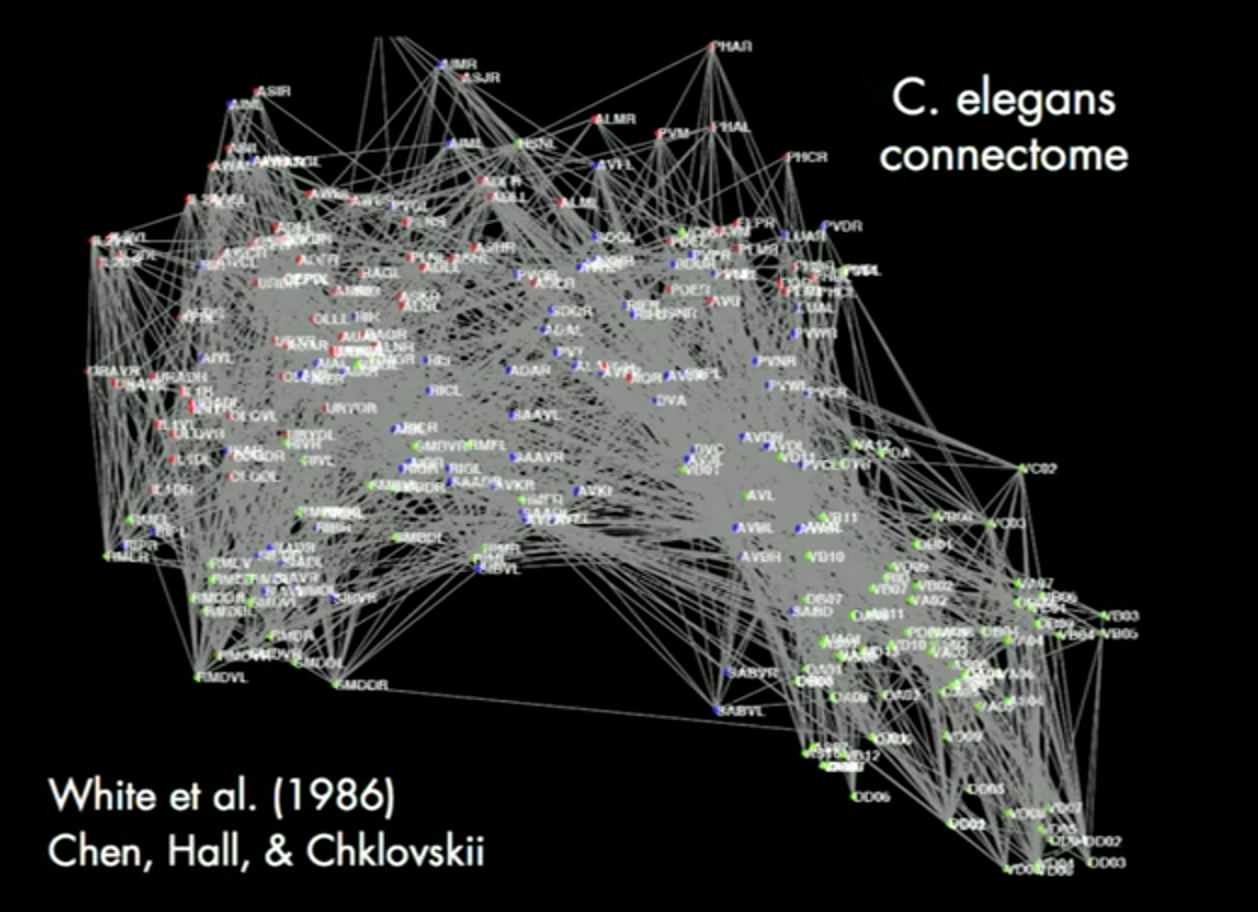
\includegraphics[width=108mm]{images/worm}
\caption{秀丽隐杆线虫的神经结构,其中的点代表了一个神经元结构并标注了相应的名称,线将神经元连接起来,表明对应的神经元通过神经纤维建立了联系}
\label{worm}
\end{figure}

White, John G 与 Southgate 等人在 1986 年时已经 利用一系列局部原始电子显微照片对秀丽隐杆线虫的神经系统的进行了完整重建\upcite{white1986structure}。经过了 30 多年的发展,Yunkyu Sohn,Myung-Kyu Choi 与 Yong-Yeol Ahn 等人于 2011 年利用基于模块化的群态检测算法发现秀丽隐杆线虫中包含了 5 个解剖簇及其对应的实验可识别功能电路,进一步揭示了生物电路如何产生更高阶的复杂行为\upcite{varshney2011structural}。即使如此,由于神经网络复杂的拓扑结构,神经科学家们仍旧未能充分探索仅仅由 300 个神经元通过突触交织而成的神经网络结构。而人类大脑由一千亿个神经元组成,神经元之间连接的数量又是神经元数量的一万倍,远比秀丽隐杆线虫的神经结构要复杂的多。因此,设计并实现自动神经元重建算法便成了探索神经结构的重要步骤之一。

Druckmann, Shaul 与 Feng 等人开发的神经元重建算法提供了准确的中线,直径,表面,体积和分支点位置,支持沿着神经元表面分析标记过的分子分布,还可以直接导出到建模软件\upcite{druckmann2014structured}。图 \ref{Druckmann} 展示了这种神经元重建算法的样例结果。Brown, Kerry M 与 Barrionuevo 等人收集了来自不同动物,脑区,神经元类型和可视化方法的六个数据集,为自动化软件所需的测试提供了基准,提高了重建的质量,同时最大限度地减少了人工的参与,极大的促进了神经元重建领域的发展\upcite{brown2011diadem}。

\begin{figure}
\centering
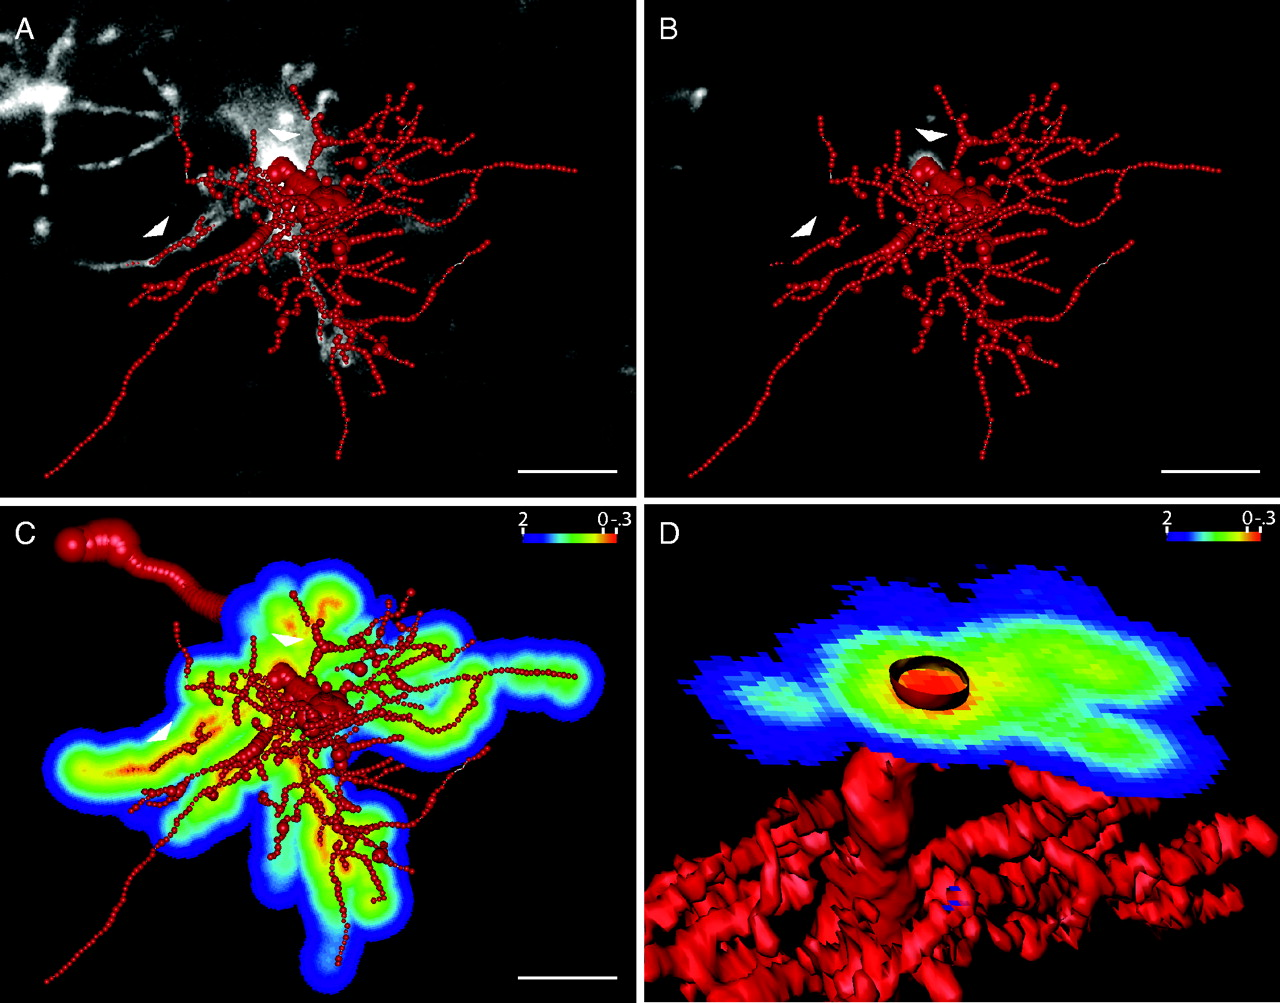
\includegraphics[width=108mm]{images/Druckmann}
\caption{Druckmann 等人的神经元重建算法的样例结果 白色的是原始神经元图像,红色的表示完成重建的神经元结构,蓝色和绿色表示对应神经元的表面概率}
\label{Druckmann}
\end{figure}

由于神经元拓扑结构的复杂性,在一些自动化重建结果的细节上仍然需要研究人员对数字重建的结果进行人工纠正和修改,以确保数字重建工作的准确性。另外研究人员需要对数字重建结果进行编辑,比如添加或删除一些网络分支等。为了便于研究人员进一步研究神经结构,探索智能产生的原因,这就需要在神经元自动重建算法的基础上建立交互式神经元重建系统,进一步提升数字重建结果的准确性,并且将多部分数字重建结果合并起来。

\section{现有系统的特点与问题}
\subsection{FARSIGHT}
FARSIGHT 的软件界面如图 \ref{FARSIGHT} 所示,图中正在编辑的是一小段神经结构,展示了用户点击位置,根节点方向,以及分支节点。
\begin{figure}
\centering
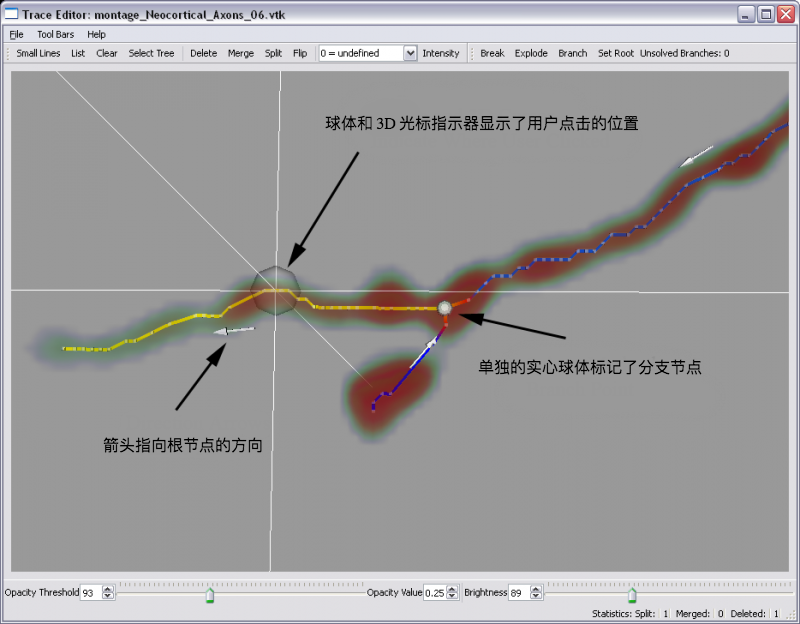
\includegraphics[width=108mm]{images/FARSIGHT}
\caption{FARSIGHT 软件运行界面 箭头指向根节点的方向,单独的实心球标记了分支节点,球体和 3D 光标指示器显示了用户点击的位置}
\label{FARSIGHT}
\end{figure}

FARSIGHT 的设计目标是保证重建结果的细节,可以快速识别重建结果的错误并能迅速纠正。FARSIGHT 利用基于模式分析辅助集群编辑(PACE)的思想,根据对自动跟踪结果的定量测量和多变量模式分析工具的分析结果,发现其中常见类型的重建错误,提高纠正重建结果的效率\upcite{luisi2011farsight}。图 \ref{FARSIGHT-res} 展示了 FARSIGHT 导出的较大规模的神经结构重建结果。

\begin{figure}
\centering
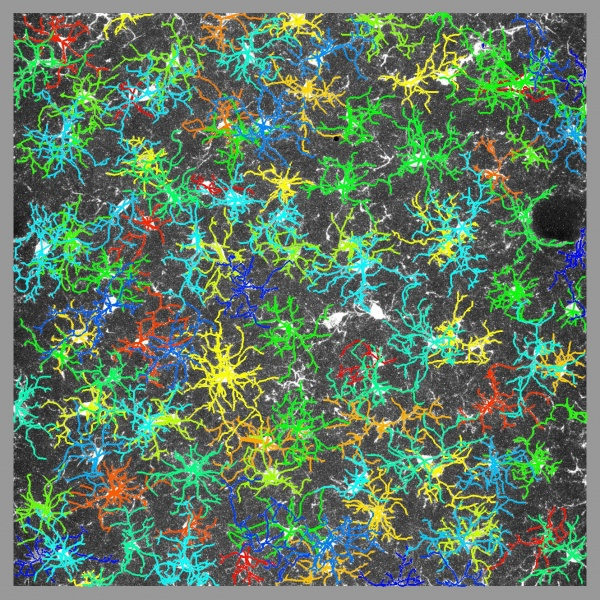
\includegraphics[width=108mm]{images/FARSIGHT-res}
\caption{FARSIGHT 导出的重建结果 每种颜色均代表了一部分神经结构}
\label{FARSIGHT-res}
\end{figure}

FARSIGHT 的缺点在于,它专注于半自动重建,对于常见的错误修改效率确实较高,但是如果遇到细小的错误,FARSIGHT 无法识别,也不提供精细化的编辑手段,需要借助于其他软件完成。

\subsection{neuTube}
neuTube 是一种基于 SWC 文件格式的神经元重建软件,同时具备 2D 和 3D 的可视化以及直观地编辑、绘制功能,允许用户高效的根据荧光图像数据重建神经元结构,并且支持编辑其他软件生成的标准神经结构的文件\upcite{Feng2014neuTube}。软件界面如图 \ref{neutube} 所示。

\begin{figure}
\centering
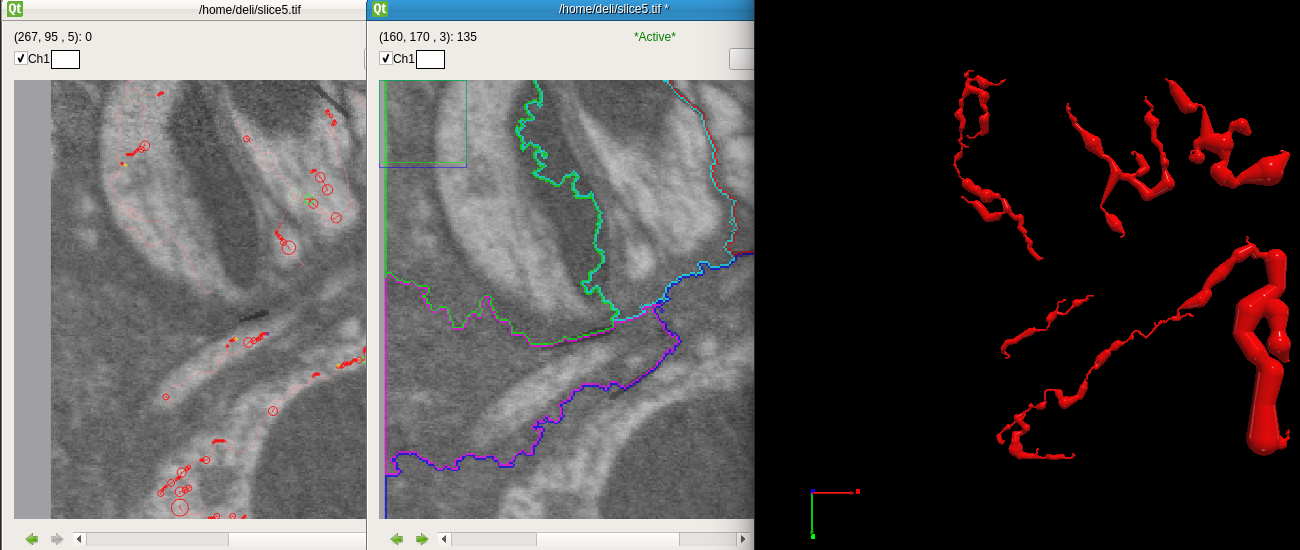
\includegraphics[width=108mm]{images/neutube}
\caption{neuTube 软件运行界面 图中展示了神经元自动重建与编辑的过程,第一个界面中红色的点是随机产生的种子点,第二个界面是根据种子点对神经元结构进行分割,图三是完成重建的神经元结构并支持用户进行纠错、编辑}
\label{neutube}
\end{figure}

虽然 neuTube 提供了 2D 和 3D 模式下精细编辑神经结构的功能,但是无法进行多人协同编辑,无法分享完成重建的结构脑胞体。

通过分析不难看出,现有的软件难以支持多名神经科学家同时进行精细化的神经结构编辑。由于神经结构的复杂性,团队合作进行神经结构的编辑,结果合并等是未来神经科学发展的趋势,因此需要设计并开发一个支持多用户协同工作的在线交互式神经元编辑平台便显得尤为重要。

\section{论文结构}
本文旨在设计并实现在线多用户的神经元网络结构编辑分享平台,利用互联网便于数据共享与交流的特点解决一些现有神经元编辑软件的问题,使得神经科学家可以便捷地进行异地,多用户协同编辑神经元网络结构,并能分享完成重建的结构脑图谱,探索神经元结构下的奥秘。由于项目涉及到数据可视化与后台服务器搭建,自然地将整个项目分成两部分,这里主要实现后台服务器的搭建,为前端可视化操作提供了有力的支持。

第一章讨论了交互式神经元重建系统的背景与意义以及现有的神经元编辑软件存在的问题,第二章讨论了项目整体架构并简单介绍所用到的技术
。第三章讨论技术实现的细节以及如何根据性能测试结果进行性能优化,第四章描述了在性能优化之后的系统整体性能,第五章讨论了接下来的工作并分析了项目中存在的不足。


    \cleardoublepage
    \chapter{整体架构与技术选型}

\section{整体架构}
项目整体结构如图 \ref{server} 所示,共分为神经信息数据库,用户信息数据库以及网络服务器三部分组成。
\begin{figure}
\centering
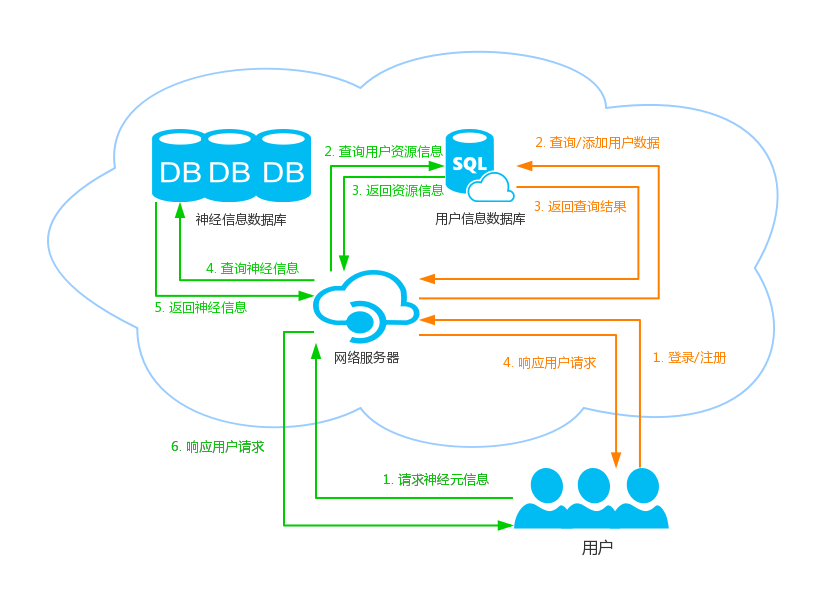
\includegraphics[width=148mm]{images/server}
\caption{项目整体架构}
\label{server}
\end{figure}
图中主要包含了两个方向的数据流,一个是用户信息数据流,另外一个是神经信息数据流。

\subsection{用户信息数据流}
用户信息数据流主要负责三件事情,一是验证用户身份,二是获取用户资源列表,三是检查用户行为是否有足够的权限。用户信息数据流可以抽象成如下几步:

1. 用户向网络服务器发送请求,登录平台或注册新用户

2. 网络服务器向用户信息数据库验证用户身份或添加新的用户信息

3. 用户信息数据库返回验证结果给网络服务器

4. 网络服务器将结果反馈给用户

\subsection{神经信息数据流}
神经信息数据流负责维护三对关系,用户和原始神经图片信息的关系,用户和数字重建结果直接的关系以及数字重建结果和原始图片信息之间的关系。神经信息数据流可以抽象成如下几步:

1. 用户向网络服务器请求神经元信息

2. 网络服务器利用用户信息数据流中保存的用户信息返回对应用户资源列表

3. 用户信息数据库返回用户资源列表给网络服务器

4. 网络服务器根据用户资源列表向神经信息数据库查询对应神经信息

5. 神经信息数据库返回对应神经信息给网络服务器

6. 网络服务器返回用户所需的神经信息用于前端的可视化展示

\section{技术选型}

\subsection{神经信息数据库}
神经信息数据库包含两部分数据,一部分是原始大脑切片显微镜图像,另外一部分是初步完成数字重建的 SWC 文件。使用 DVID 作为数据库,储存这些信息。DVID 是一个分布式面向图像的数据服务,主要用于图像分析与可视化\upcite{dvid}。DVID 有如下特点:

1. 便于扩展数据类型,允许用户根据数据特点加速访问速度,减少储存空间,提供方便的 API。这为储存数字重建结果提供了便利。

2. 为分布式数据储存提供了类似于 GIT 的版本控制系统,在此基础之上我们可以解决多用户同时编辑产生冲突的问题。

3. 方便连接其他 API 如 Google BrainMaps 和 OpenConnectome 等。

4. 支持多分辨率图像数据,使得用户可以在不同尺度下观察图像信息。

在 DVID 的基础上,构建出原始大脑切片显微镜图像与数字重建结果的储存仓库,将数据储存抽象成数据存储服务,使得可以专注于完成核心算法和逻辑。

\subsection{用户信息数据库}
用户信息数据库包含多用户管理以及用户资源管理。使用 PostgreSQL 数据库储存这部分信息。PostgreSQL 最初由加州大学伯克利分校计算机系开发完成。在支持大部分 SQL 标准之上,提供了许多诸如复杂查询,多版本并行控制,事物完整性等现代特性\upcite{stonebraker1991postgres}。由于 PostreSQL 对标准 SQL 支持度较高,可以方便的和 DVID 联系起来,将用户信息和原始图像信息,数字重建结果对应起来。利用 PostgreSQL 支持的储存过程,事物以及多版本并行控制特性,我们可以方便的实现分布式,多用户实时编辑平台,并解决多用户同时编辑可能产生冲突的问题。

\subsection{网络服务器}
采用 Node.js 和 Express 完成网络应用开发。Node.js 是一个基于 Chrome V8 引起的 JavaScript 的运行环境。Node.js 使用了一个事件驱动、非阻塞式 I/O 的模型,使其轻量又高效\upcite{tilkov2010node}。Express 是一个基于 Node.js 平台的极简、灵活的 web 应用开发框架,提供丰富的 HTTP 快捷方式和任意排列组合的 Connect 中间件,帮助快速、简单的创建健壮、友好的 API。
    \cleardoublepage
    \chapter{平台搭建与性能调优}
\label{chap3}

\section{数字重建结果的表示}
为了储存完成数字重建的结构脑胞体,并为前端的可视化操作提供相应的 API 支持,需要定义一种存储结构脑胞体的格式,这种格式需要满足如下特点:

1. 便于储存

2. 便于前后端之间传输

3. 支持对神经元的操作,并支持历史版本记录

根据“所见即所得”的原则,Peng, H. 和 Long, F. 等人设计出了 SWC 格式\upcite{Peng2011Proof}。SWC 的结构清晰,可操作单元定义名曲,用户输入与编辑操作有清晰明确的对应关系。在 SWC 格式的基础上,研究人员可以方便、直观地纠正自动化数字重建结果的错误,添加新的分支或删除已有分支。

Feng, Linqing 与 Zhao 等人用点集高度抽象了结构脑胞体,将其表示成树状结构,进一步提升了对神经元结构的表达能力\upcite{Feng2014neuTube}。用点集定义结构脑胞体如下所示:$\{ n_i = (x_i, y_i, z_i, n_j) | i = 1,..., N, j = 0,..., N, i \neq j, x_i, y_i, z_i, r_i \in R \}$,点与神经元之间的连接构成了一个树形结构,合法的神经元结构不允许出现环。每一个点 $n_i$,都是一个中心在 $(x_i, y_i, z_i)$,半径为 $r_i$ 的球。$n_0$ 是一个空点,用来表示神经结构的根,$n_j$ 表示 $n_i$ 的父节点。从 $n_i$ 到 $n_j$ 表示一段向上的路径,这可以用一个数组 $(n_{k_1},...,n_{k_n})$ 来表示, 其中 $n_{k_i+1}$ 代表 $n_{k_i}$ 的父节点 $k_1 = i, k_n = j$。在这个模型中,基础结构单元是点,点定义了神经元结构的储存方式以及交互方式。

但是仅仅定义结构脑胞体无法满足多用户编辑的需求。因为在多用户同时编辑的时候,可能存在操作冲突即两个用户同时对相同的结构脑胞体进行操作,这是需要区分出不同用户的操作,因此需要进一步将结构脑胞体的操作抽象出来并储存在数据库之中。

假设 $S_1$ 和 $S_2$ 是两个点集,对于一个神经结构的操作可以定义为:
$$f(S_1) = S_2$$
举例来说,$f(S_1)= \phi$, 式中 $\phi$ 代表空集,$f$ 表示将点集 $S_1$ 变换成了空集,意味着将点集 $S_1$ 删除,因此 $f$ 定义了删除操作。
在定义接下来的操作之前,需要明确点的表示方式。简单来讲,点的表示只需要记录位置信息与父节点即可,但是为了提高遍历节点的效率,在点的表示中加入了一些冗余信息,例如子节点与兄弟节点。$n=(G(n), P(n), C(n), S(n))$, 其中 $G(n) = (x(n), y(n), z(n), r(n))$。$n$ 定义了一个在$(x(n), y(n), z(n), r(n))$ 处,半径为$r(n)$,父节点为 $p(n)$ 的节点 $n$。 $n$ 的第一个子节点为 $C(n)$,下一个兄弟节点为 $S(n)$。查询子节点时,这样的表示方式只需要检查它的第一个子节点并遍历其兄弟节点即可,而在非冗余结构中,每个节点只与其父节点相连,算法需要检查树中的每个节点。

根据上述对操作的抽象,可以将编辑节点 $n$ 的值可以用修改对应的元组来定义。对 $G(n)$ 的改变称为几何变换,对 $P(n), C(n), S(n)$ 的变换成为结构变换。几何变换是较为直观的,仅仅代表了神经元在空间上的位移,图 \ref{gem} 展示了最简单的几何变换。结构变换改变了结构脑胞体之间相互连接的关系,图 \ref{stru} 展示了一个结构变换,此时单独修改编辑过的神经元对应的元组信息是不够的,会造成非法的结构脑胞体。例如仅改变 $P(n)$ 会打破 $P(C(n)) = n, P(n) = P(S(n))$ 的规则。为了避免这样的问题,需要进一步对结构脑胞体的结构操作在不同层次上进行抽象。

\begin{figure}[!ht]
\centering
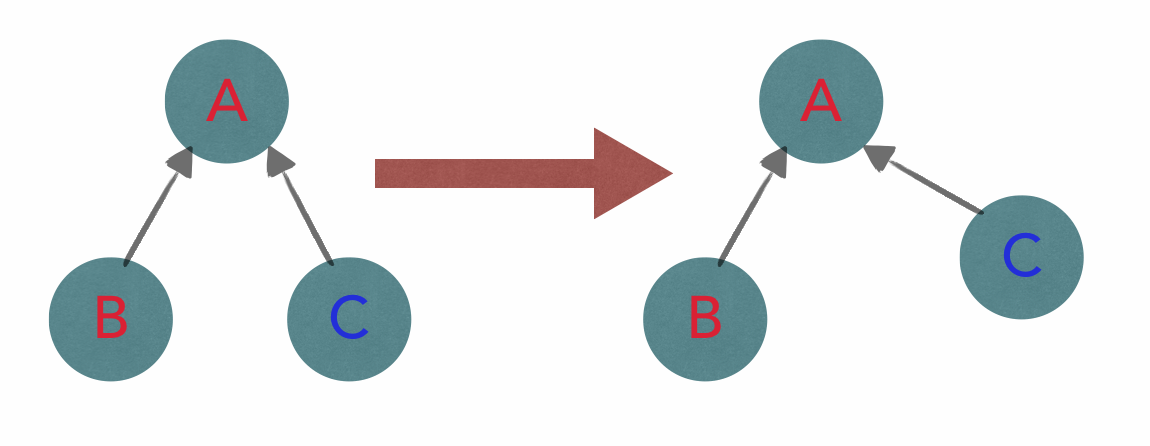
\includegraphics[width=148mm]{images/gem}
\caption{由三个神经元组成的几何变换实例 根节点是神经元 A,神经元 C 的位置向右上方发生了一些改变,此时只需要改变表示神经元 C 元组的 G(n) 部分即可,神经元 A,B 不需要改变}
\label{gem}
\end{figure}

\begin{figure}[!ht]
\centering
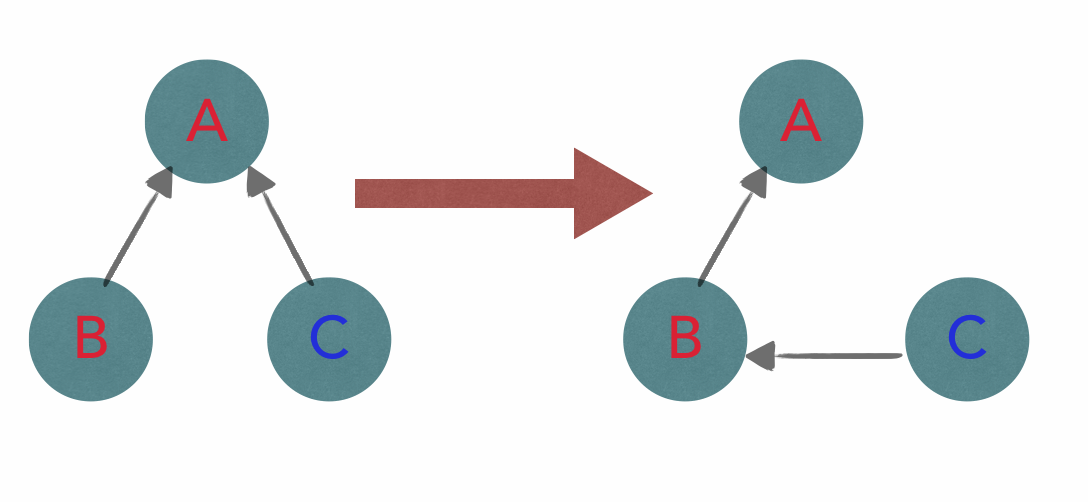
\includegraphics[width=148mm]{images/stru}
\caption{由三个神经元组成的结构变换实例 根节点是神经元 A,神经元 C 的
父节点从神经元 A 变成了神经元 B,此时只需要改变表示神经元 C 元组的 P(n) 会造成非法的神经元结构,需要相对于的调整神经元 A 与神经元 B 的元组信息}
\label{stru}
\end{figure}

第一层次操作包含三个基本操作, 分别表示了对 $P(n), C(n), S(n)$。这三种操作可以用以下公式定义:
$$f_p(\{n\}|n') = f_p(\{G(n), P(n), C(n), S(n)\}|n' = \{(G(n), n', C(n), S(n))\})$$
$$f_c(\{n\}|n') = f_c(\{G(n), P(n), C(n), S(n)\}|n' = \{(G(n), P(n), n', S(n))\})$$
$$f_s(\{n\}|n') = f_s(\{G(n), P(n), C(n), S(n)\}|n' = \{(G(n), P(n), C(n), n')\})$$
在这个层次上,仅仅表示了三种最基本的结构操作,分别是修改子节点,修改父节点与修改兄弟节点,这一层次的操作只修改了被编辑神经元的数据,无法保证结构的合法性。

第二层次操作将三种基本的操作进行了封装,保证了结构的合法性。假设 $F_{p_0}(n)$ 代表将节点 $n$ 的父节点设为 $n_0$, 即空节点, 如果$C(P(n)) = n$,即 $n$ 是父母的第一个子节点,
$$
F_{p_0}(n) =
\left\{
\begin{aligned}
f_s(\{n\} | n_0) \circ f_p(\{n\} | n_0) \circ f_c(\{P(n)\} | S(n)), C(P(n)) = n\\
f_s(\{n\} | n_0) \circ f_p(\{n\} | n_0) \circ f_c(\{S^{-1}(n)\} | S(n)), otherwise
\end{aligned}
\right.
$$
其中,$f \circ g$ 代表一个复合操作,$S(S^{-1}(n)) = n$。为了更清楚的定义一个单节点,在不增加歧义的情况下,$F_{p_0}(n)$ 被定义为一个函数而不是一个点集。
设置父节点的操作被定义为
$$F_p(n|n') = f_c(\{C(n')\}|n) \circ f_s(\{n\}|C(n'))  \circ f_p(\{n\}|n') \circ F_{p_0}(n)$$
设置 $n$ 作为 $n{}'$ 的第一个子节点虽然可以用其他的操作合成出来,但是在实践中,定义更多的操作对于储存以及前后之间的交互提供了极大的便利。
$$F_s(n|n') = f_s(\{n'\}|n) \circ f_s(\{n'\}|S(n))  \circ f_p(\{n'\}|P(n)) \circ F_{p_0}(n')$$
对于图 \ref{stru} 中所示的结构变换所对应的第三层次操作包含了三个第一层次的操作:

1. 修改神经元 C 的父节点

2. 修改神经元 B 的兄弟节点

3. 修改神经元 B 的子节点

而对于图 \ref{stru2} 中所示的结构变化与图 \ref{stru} 所示的改变对称。但是由于神经元 C 是根节点神经元 A 的第一个子节点,所以与图 \ref{stru} 包含的第一层次操作不同,由 4 个第一层次操作构成:

1. 修改神经元 C 的父节点

2. 修改神经元 B 的子节点

3. 修改神经元 A 的子节点

4. 修改神经元 C 的兄弟节点

\begin{figure}[!ht]
\centering
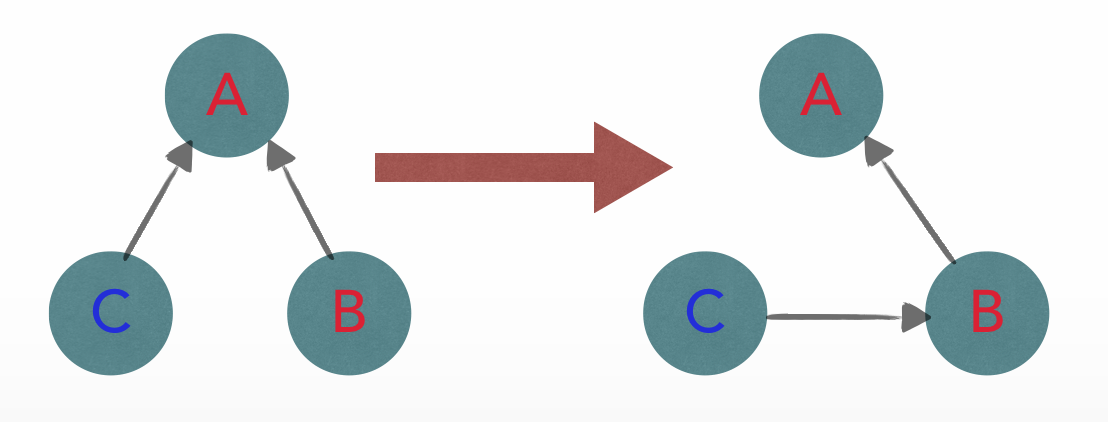
\includegraphics[width=148mm]{images/stru2}
\caption{另一种由三个神经元组成的结构变换实例 根节点是神经元 A,神经元 C 作为根节点神经元 A 的第一个子节点在第二层次的操作需要修改 神经元 A 的子节点}
\label{stru2}
\end{figure}

通过对简单操作进行抽象,使得不需要关注与有大量细节并且可能造成非法结构的第一层操作,避免了许多可能出现的问题,并且减少了一些操作合法性的检查,减少了计算量。

第三层次由一组复合操作组成,其中包括任何第二层次的操作复合而成的操作。将一个操作分解为基本操作有助于保证编辑操作的有效性。更重要的是,分解基础操作有助于实现撤销和重做任意操作。撤销操作要求撤消任意复杂度的操作。例如,删除的逆运算需要恢复多个相邻的节点。直接推导逆操作不仅需要大量的工作,也容易导致很难绘制错误。将一个操作分解为一系列基本操作之后,这样可以很容易构造撤消操作的逆转序列。

第三层操作由第二层复合而来,第二层操作由第一层复合而来,而第一层操作只包含三种情况,这样便可以用三种操作来表示结构
结构变换,加上可以直观的用三种操作表示的几何变换,共可以用六种操作表示所有的对神经元结构的操作。这样便可以针对这六种简单操作设计不同的 API 供前端调用,使得针对操作的特点进行优化成为了可能。根据第三层次的抽象,流程处理用户的编辑请求的算法如 \ref{a-con} 所示。

\begin{algorithm}
  \label{a-con}
  \caption{将用户编辑操作转换成操作序列}
  \begin{algorithmic}[1] %每行显示行号
    \STATE{获取可用编辑操作列表}          // 第二层次操作
    \IF{有所需的编辑操作} 
      \STATE{选取所需编辑操作} 
    \ELSE
      \STATE{用户自定义编辑操作}     // 通过组合第一层次操作构建第二层次操作
      \WHILE{自定义操作不合法} 
        \STATE{根据提示修改掉操作不合法的地方}
      \ENDWHILE
      \STATE{保存用户的自定义编辑操作}
    \ENDIF
    \STATE{将编辑操作储存到数据库中}
    \STATE{将编辑操作转换成第一层次操作}
    \STATE{修改结构脑胞体}
  \end{algorithmic}
\end{algorithm}

这里值得注意的是需要储存在数据库中的是第二层次的编辑操作,作用在结构脑胞体上的是第一层次操作。考虑到需要支持撤销,多用户操作合并等功能,保存第一层次操作无法保证编辑操作的完整性,为实现这些功能增加了难度。另外,如果只撤销了编辑操作的一部分很可能造成非法的结构脑胞体。而编辑操作作为一种高层次的抽象,无法直接作用在结构脑胞体之上,需要转换成更底层的可以直接反应结构脑胞体元组之上的第一层操作。

\section{数据库结构设计}

\subsection{用户信息数据库}
为了实现多用户管理以及用户资源管理,共设计实现了三张数据表,分别是用户信息表,原始图像数据表以及结构脑胞体数据表。这些数据表主要用户实现用户信息数据流,并和 DVID 储存的神经信息数据库相互关联,为神经信息数据流提供了资源管理和权限控制等相应的支持。

1. 用户信息表
用户信息表如表 \ref{user-table} 所示,共有三个字段,分别储存了用户名,密码和用户保证账户安全的盐值。
\begin{table}
\centering
\caption{用户信息表}
\begin{tabular}{|c|c|c|}
			   \hline
                 字段名 & 数据类型 & 备注 \\
               \hline
                 username & STRING & 主键 \\
               \hline
                 password & STRING &  \\
               \hline
                 salt & UUID & 用于保证用户账户安全 \\
               \hline
             \end{tabular}
             \label{user-table}    
\end{table}

2. 原始图像数据表
原始图像数据表如表 \ref{image-table} 所示,共有三个字段,分别储存了创建者,图像名和权限控制的用户角色。

\begin{table}
\centering
\caption{原始图像数据表}
\begin{tabular}{|c|c|c|}
			   \hline
                 字段名 & 数据类型 & 备注 \\
               \hline
                 username & STRING & 创建者,外键,用户信息表中的 username \\
               \hline
                 image & STRING &  \\
               \hline
                 role & STRING & 用于权限控制 \\
               \hline
             \end{tabular}
             \label{image-table}    
\end{table}

3. swc 数据表
原始图像数据表如表 \ref{swc-table} 所示,共有五个字段,分别储存了创建者,图像名,创建时间,swc 文件名以及用户评论。根据创建时间,可以建立同一图像下 swc 文件的拓扑顺序,为多用户同时编辑以及合并冲突分支提供了基础。

\begin{table}
\centering
\caption{原始图像数据表}
\begin{tabular}{|c|c|c|}
			   \hline
                 字段名 & 数据类型 & 备注 \\
               \hline
                 username & STRING & 创建者,外键,用户信息表中的 username \\
               \hline
                 image & STRING & 原始图像名,外键,原始图像数据表中的 image \\
               \hline
                 createdAt & TIME & 创建时间 \\
               \hline
                 swc & TEXT & swc 文件名 \\
               \hline
                 comments & STRING & 备注 \\
               \hline
             \end{tabular}
             \label{swc-table}    
\end{table}

\subsection{神经信息数据库}
神经信息数据库储存了原始神经切片图像信息,完成数字重建的结构脑胞体以及用户的编辑操作。DVID 提供了 imagetile 和 Key-Value 两种类型的数据类型,原始神经切片图像信息选择使用 imagetile 数据类型,结构脑胞体以及用户的编辑操作选择了 Key-Value 数据类型。

1. 原始神经切片图像信息
如图 \ref{dvid} 所示,对于 imagetile 类型的数据提供了数据预览功能。图中展示的神经组织在 z 方向上是一层层的切片,在 xy 方向上是完整的一整张图片。由于在精细神经编辑编辑时需要获取局部信息,并对局部信息进行放大,因此提供的 API 需要提供获取图像的范围以减少数据的传输量,提升响应速度。

\begin{figure}[!ht]
\centering
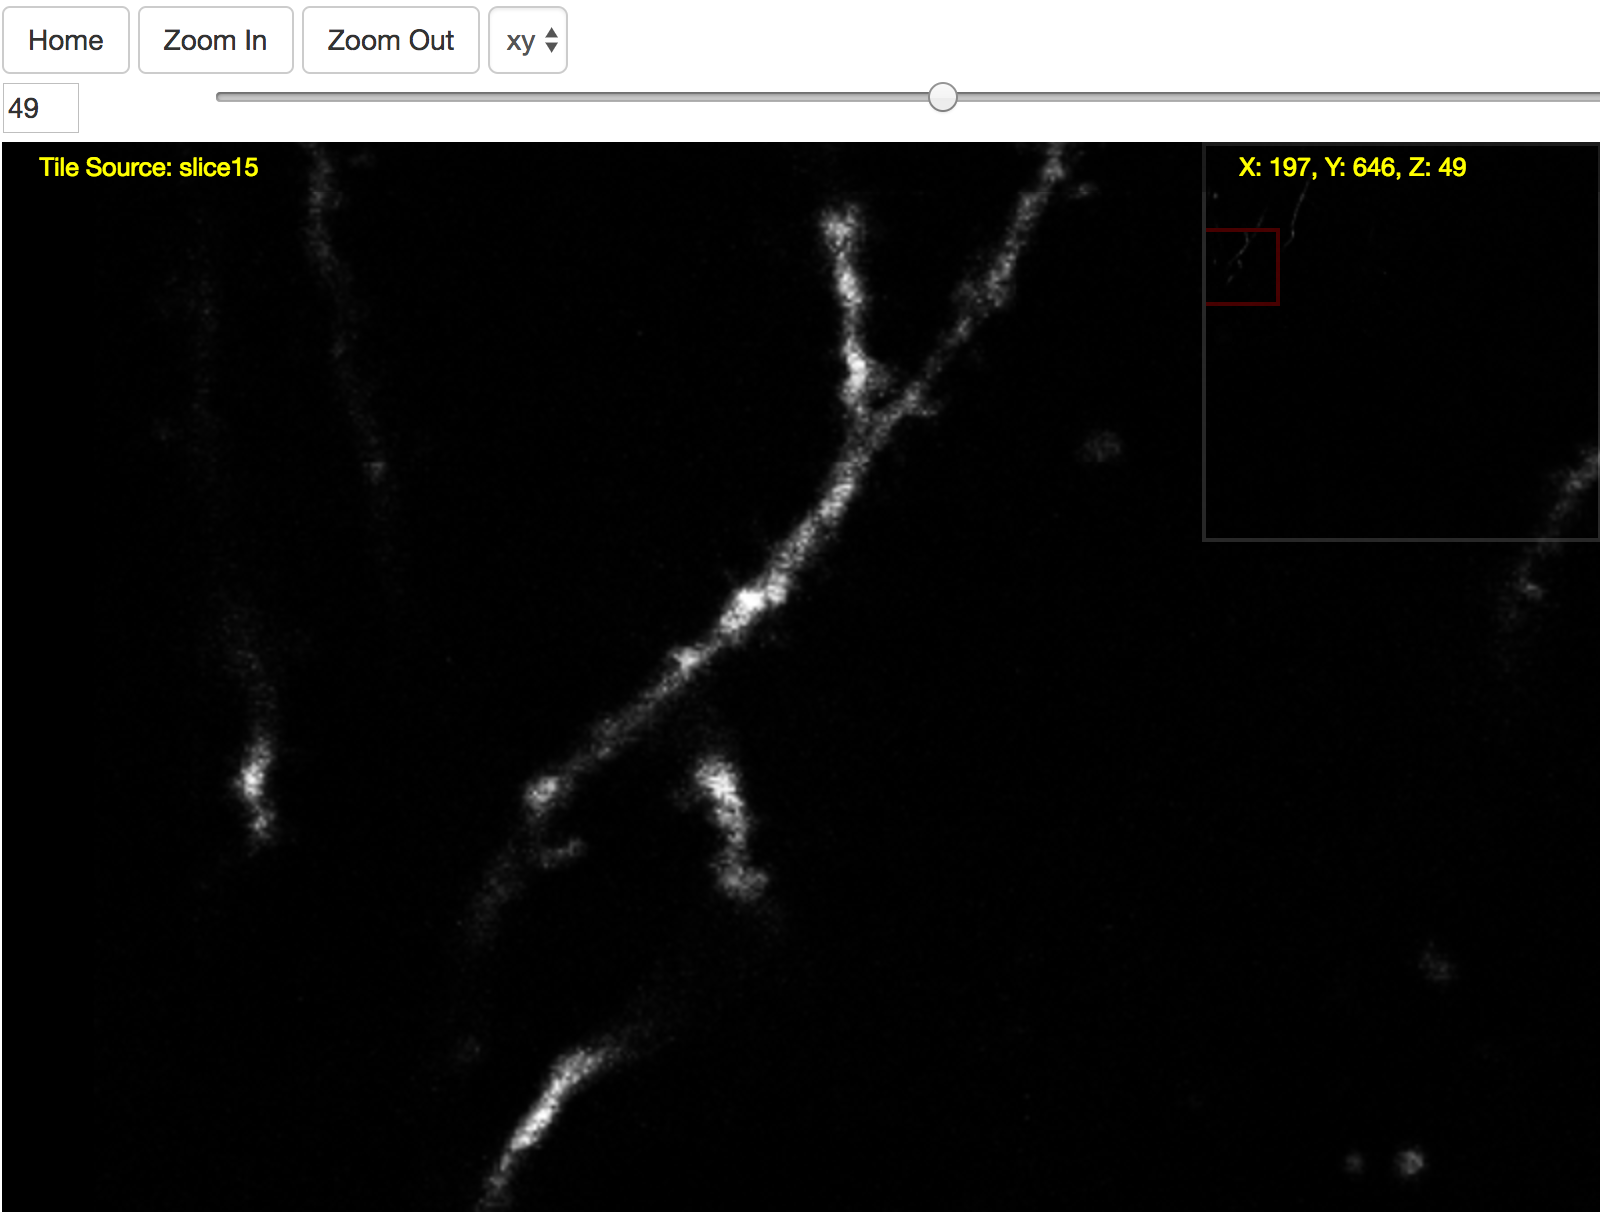
\includegraphics[width=108mm]{images/dvid}
\caption{DVID 对于 imagetile 类型数据提供的数据预览功能 图中展示了一部分神经组织}
\label{dvid}
\end{figure}

2. 结构脑胞体与用户的编辑操作
由于完成数字重建的结构脑胞体结构多样,数据量较大,涉及多种可能进行的编辑操作且需要支持用户自定义编辑操作,传统的结构化数据库较难支持这样的功能。DVID 支持的 Key-Value 数据类型提供了较为简单的 NoSQL 储存服务,满足了目前的需要。NoSQL 系统的一个关键特性是“无共享”,这使得 储存服务,满足了目前的需要。NoSQL 系统可以在许多服务器上复制并分割数据,这使得 NoSQL 系统每秒可以支持大量简单的读/写操作\upcite{cattell2011scalable},这正好符合结构脑胞体与用户的编辑操作数据量大,无固定格式的特点。

\section{基础平台的搭建}
在确定了结构脑胞体的表示方式并完成了数据库结构的设计之后,基础平台的搭建更多是工程上的考虑与工作。项目初期针对可能会涉及到的技术做了广泛而细致的调查与研究,最终确定了在上一章中的技术选型,选择了合理且先进的技术使得开发工作完成的十分顺利,可以将时间用在测试与性能调优。

\subsection{跨浏览器兼容}
由于网络浏览器市场竞争激烈,浏览器的开发速度非常快,新增功能不需要供应商之间的协调。引入新功能的优先级通常会优先于错误修复,导致浏览器不稳定,不符合 Web 标准,频繁崩溃并且具有许多安全漏洞。为了标准化 JavaScript,Ecma International 在 ECMA-262 和 ISO / IEC 16262中提出了 ECMAScript \upcite{ecma1999262}。 在项目中希望使用 ECMAScript 来编写网站,使平台更加符合互联网标准。然而在目前的互联网环境中,各个浏览器对 ECMAScript 的支持并不好,很多的神经学家依旧在使用较为老旧的浏览器,ECMAScript 在这样的环境中无法运行。图 \ref{es5} 展示了一些较为老旧的浏览器对 2009 年推出 ECMAScript5 的支持程度,IE7 完全不支持,甚至是较为现代的 Chrome 浏览器也没有完全支持。Juriy Zaytsev 等人详细讨论了不同浏览器对不同版本 ECMAScript 中每个特性的支持程度,各个浏览器的兼容性不容乐观\upcite{kangax}。HTML 和 css 也存在这样的问题,很多现代的特性在老旧的浏览器中无法使用。

\begin{figure}[!ht]
\centering
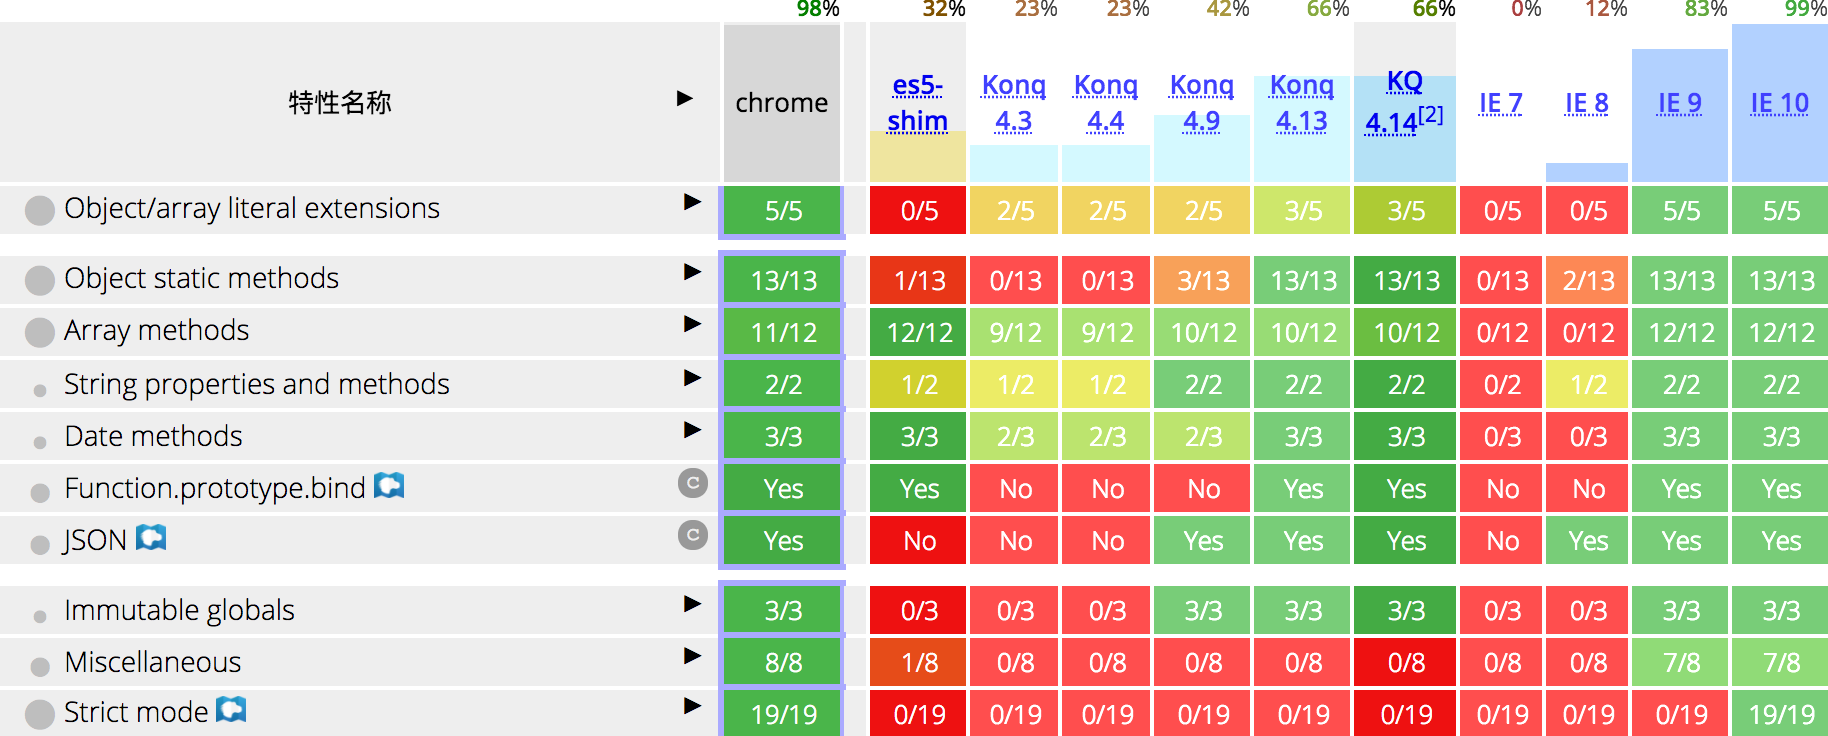
\includegraphics[width=148mm]{images/es5}
\caption{部分浏览器对 ECMAScript5 的支持程度}
\label{es5}
\end{figure}

为了解决这个问题,既可以让前端可视化人员能使用先进的特性,也可以保证在老旧的浏览器环境中可以正常运行,需要将现代的语法标准针对每种不同的浏览器,转换到每种浏览器自己的标准上。配合使用 webpack \upcite{webpack}这一工具,针对使用率较高的浏览器的标准完成了这一工作。前端可视化人员可以随意的使用最先进的 支持的并不好,很多的神经学家依旧在使用较为老旧的浏览器,ECMAScript 7,HTML 5 以及 CSS 3 等技术来完成可视化和神经结构编辑任务而不用考虑老旧的浏览器是否支持这些技术,经过 webpack 及其一些列定制化的插件\upcite{loader, uglify},将其转换到不同浏览器自己的标准上,较为完善的解决了这一问题。图 \ref{webpack-flow} 描述了 webpack 的工作流程,将各种所需的依赖打包在一起,通过不同的插件将浏览器不支持的新特性转换到最基础的语法上,保证了各个浏览器的兼容性。在转换的过程中还实现了代码混淆和打包压缩,一定程度上提高了安全性和效率。

\begin{figure}[!ht]
\centering
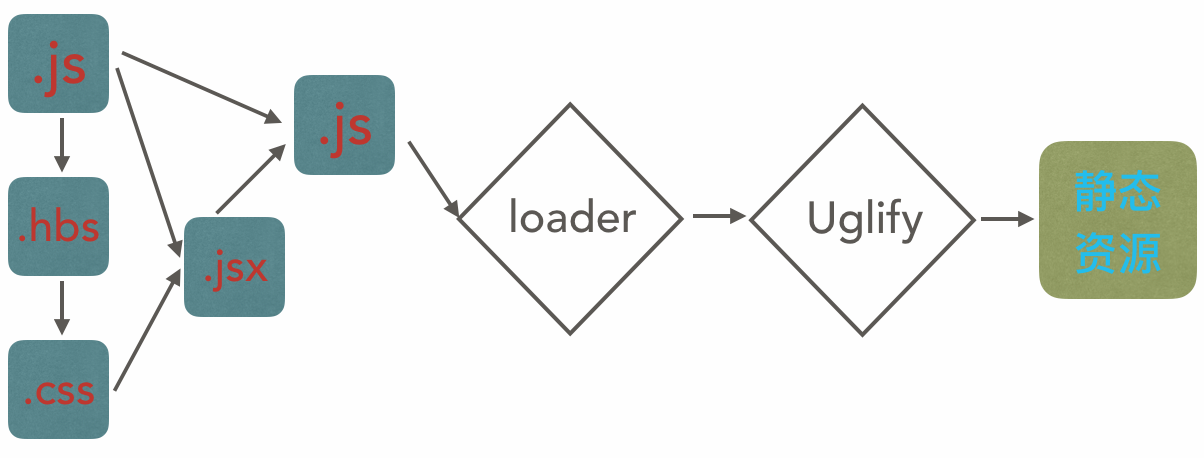
\includegraphics[width=148mm]{images/webpack}
\caption{webpack 的处理流程,.js 表示所需要的 JavaScript 模块,.hbs 表示网页模板系统,.jsx 表示 React \upcite{react} 的各个组件,.css 表示网站样式资源。中间的 loader 和 Uglify 表示代码转译,混淆和压缩的插件。右边的静态资源文件代表发送向客户端的文件。}
\label{webpack-flow}
\end{figure}

\subsection{原始图像信息传输}
由于在编辑神经元结构的过程中需要对照原始图像信息,而每一张图片仅仅代表神经组织的一个切片,如果在 3D 模式下进行编辑会设计到许多张原始图片,因此图像信息的传输占据了网络服务器服务器绝大多数的流量。因此实现原始图像信息的传输在平台搭建的过程中占据了重要地位。

原始神经元图像,如图 \ref{neu} 所示,有两个特点:

1. 背景面积大,实际的神经元组织在图像中的面积较小。

2. 绝大多数图像是灰度图,数据只有一个通道,甚至有部分图像是黑白图像,只有 0 和 1。

\begin{figure}[!ht]
\centering
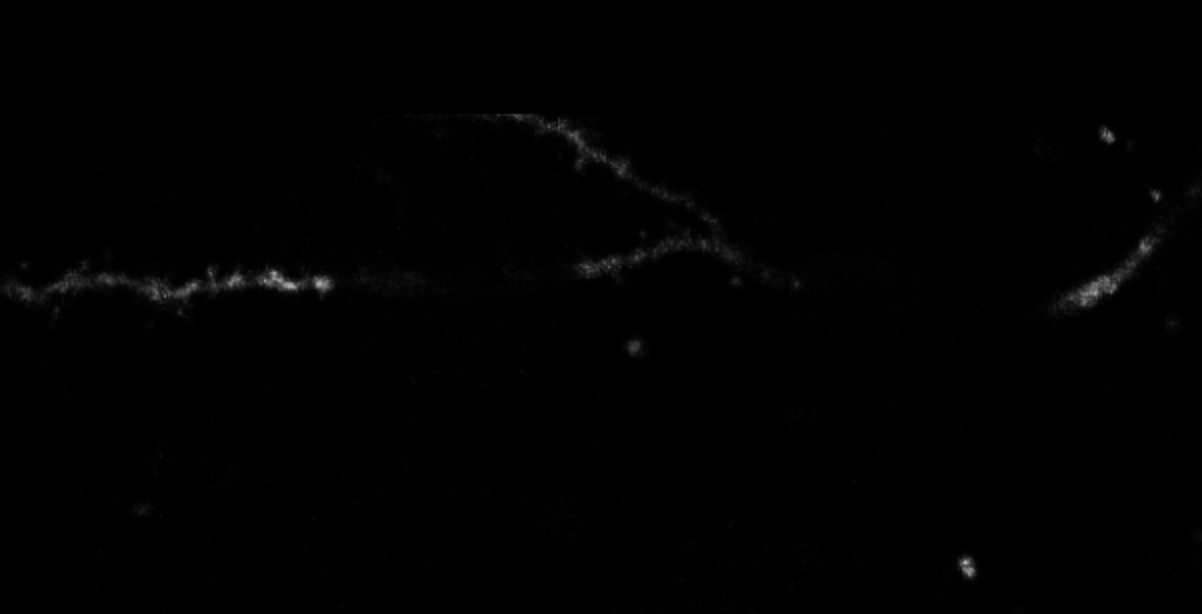
\includegraphics[width=108mm]{images/neu}
\caption{原始神经元图像样例}
\label{neu}
\end{figure}

针对神经元图像的这个特点,可以针对性的传递图片中的神经元组织,忽略掉大面积的黑色背景,这样做会大大降低所需要传递的数据量。由于神经元组织在荧光显微镜下显示为白色,图片背景为黑色,因此神经组织的表示如下:

$$F = {f | f \in image ~~ \&\& ~~ f > threshold} $$

背景表示如下:

$$B = {b | b \in image ~~ \&\& ~~ b \leq threshold} $$

对前景神经组织采用 CRS \upcite{wiki:crs}的方式,采用 A 与 IA 两个数组储存。

但是这样做一方面需要判断图片中的神经组织,增大后端服务器的计算量,另一方面对于一些不同显微镜下的图片神经元在图像中的比例较大,这种优化方式甚至会加大数据传输量。最终采取的解决方案是在后端服务器计算资源空闲的时候对原始图像信息进行处理,对于处理完毕且图像中神经元组织较小的图片只传输神经元组织信息,反之传递原始图像,具体过程如算法 \ref{a-img-pro} 所示。。这样做在绝大多数场景下取得了较高的性能。

\begin{algorithm}
  \label{a-img-pro}
  \caption{图像信息发送过程}
  \begin{algorithmic}[1] %每行显示行号
    \STATE{读取用户请求}
    \STATE{从 DVID 中读取对应的神经元图像信息}
    \IF{图像缓存中存在处理过的图像信息} 
      \STATE{发送缓存中的图像信息} 
    \ELSE
      \IF{图像中背景占据绝大多数位置} 
        \STATE{将图片发送到服务器处理队列,在服务器空闲时进行处理} 
      \ENDIF
      \STATE{发送原始图像信息}
    \ENDIF
  \end{algorithmic}
\end{algorithm}

\section{平台硬件架构}
在软件编写完成之后,共使用三台计算机作为网络节点部署了在线交互式神经元编辑平台。其中一台计算机部署神经信息数据库和用户信息数据库,另外两台部署网络应用服务器用于负载均衡。每台计算机的详细配置如下:

1. 操作系统: Ubuntu 16.04.2 LTS (GNU/Linux 4.4.0-72-generic x86\_64)

2. 中央处理器: Intel(R) Xeon(R) CPU E5-2620 v2 @ 2.10GHz

3. 内存:63149 MB

4. 网卡:Ethernet controller: Broadcom Corporation NetXtreme II BCM57800 1/10 Gigabit Ethernet * 4

5. 硬盘:1.75 TB 机械硬盘

\section{性能优化}

在测试平台搭建完成后,使用 Gatling\upcite{gatling} 进行了压力测试,测试结果如图 \ref{origin} 所示。测试中一共模拟了 100 名用户同时访问平台,每位用户模拟进行不同的操作共计 301 次,所有用户共计 30100 次操作,平均每秒进行 2508.333 次操作。

\begin{figure}[!ht]
\centering
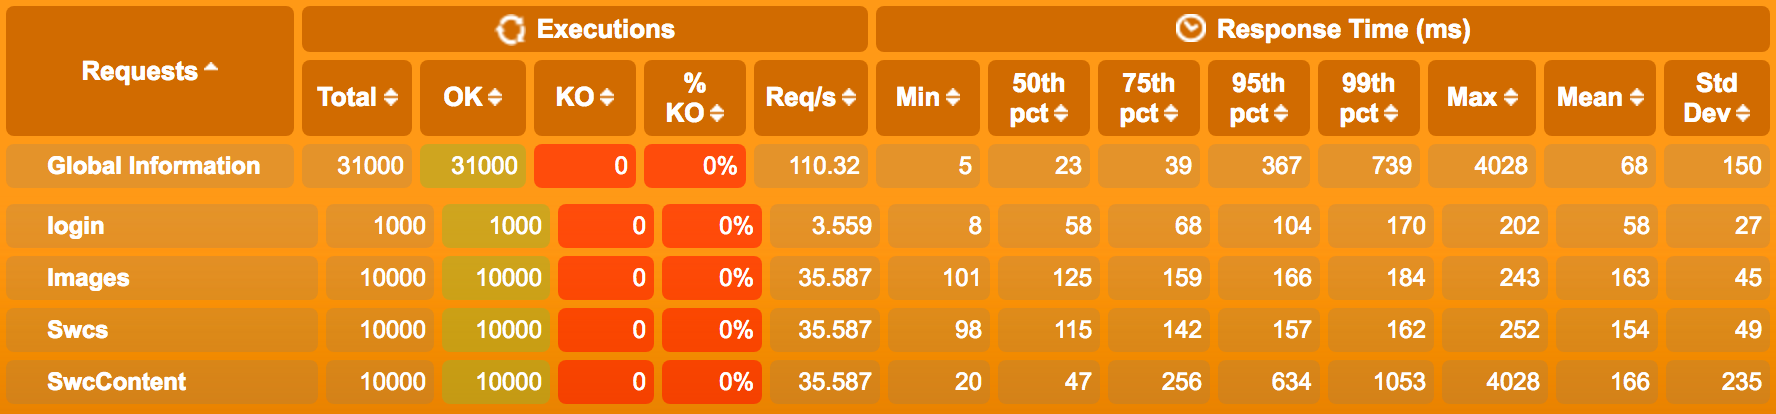
\includegraphics[width=108mm]{images/origin}
\caption{未经过任何优化的性能数据。图中 Login 代表用户登录的请求, Images 代表获取用户原始图像列表相关 API 的响应时间,Swcs 代表用户对神经元结构进行操作的相关 API 的响应时间,SwcContent 代表用户获取结构脑胞体的响应时间。}
\label{origin}
\end{figure}

\subsection{优化获取结构脑胞体的响应时间}
从图 \ref{origin} 中可以看出获取结构脑胞体的响应时间较长,最长响应时间甚至达到了 4028ms,这对于用户来说是可以明显感受到的卡顿,甚至是不可接受的卡顿,这使得需要对获取结构脑胞体的 API 进行性能优化。考虑到这个 API 需要传输大量的数据,响应时间过长是由传输数据量较大导致的性能问题,可以考虑从减少传输的数据量入手。经过调查相关技术,最终采用两种方式进行优化。第一个方案是采用浏览器端的数据库 indexDB 进行缓存\upcite{network2013indexeddb},将已经获取过的结构脑胞体储存在客户端中,减少了向服务器的请求次数。另一方面,根据 Mogul, Jeffrey C 等人提出的在 HTTP 中提出的有关使用的编码和压缩方式的技术对结构脑胞体的数据进行了压缩 \upcite{mogul1997potential},使得传输的数据量更小。结合这两点,将获取结构脑胞体的平均响应时间从 166ms 降低到了 17ms,降低了 89.75\%,具体数值如图 \ref{swccontent},详细的响应时间分布如图 \ref{swcdic} 所示,获取结构脑胞体的响应时间大大降低。图 \ref{res-time} 描述了经过优化的获取结构脑胞体响应时间随时间的变化,高响应时间的请求集中在开始时,后续的请求响应时间几乎为零,这显示了使用 indexDB 对数据进行缓存所带来的巨大性能提升。

\begin{figure}[!ht]
\centering

\includegraphics[width=108mm]{images/swccontent}
\caption{经过优化的获取结构脑胞体响应时间,从 166ms 降低到了 17ms,降低了 89.75\%}
\label{swccontent}
\end{figure}

\begin{figure}[!ht]
\centering
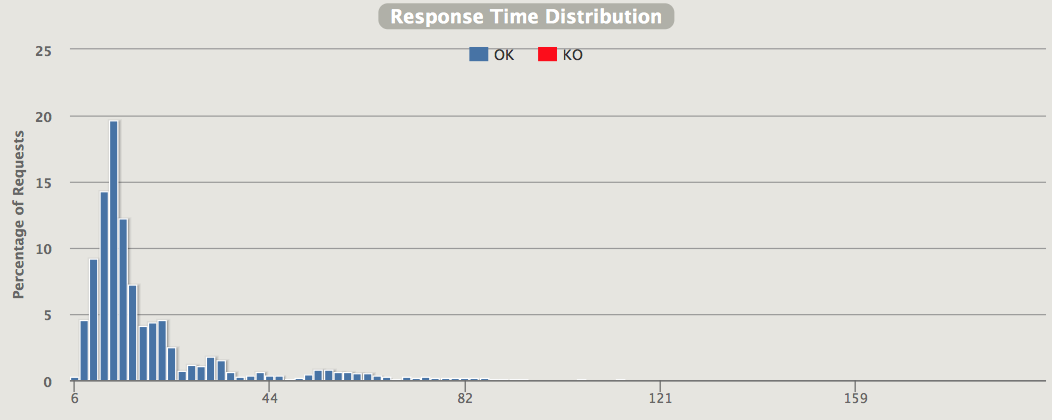
\includegraphics[width=108mm]{images/swcdic}
\caption{经过优化的获取结构脑胞体响应时间分布,绝大多数的响应时间在 6~44 ms 之间,用户感受不到明显的卡顿}
\label{swcdic}
\end{figure}

\begin{figure}[!ht]
\centering
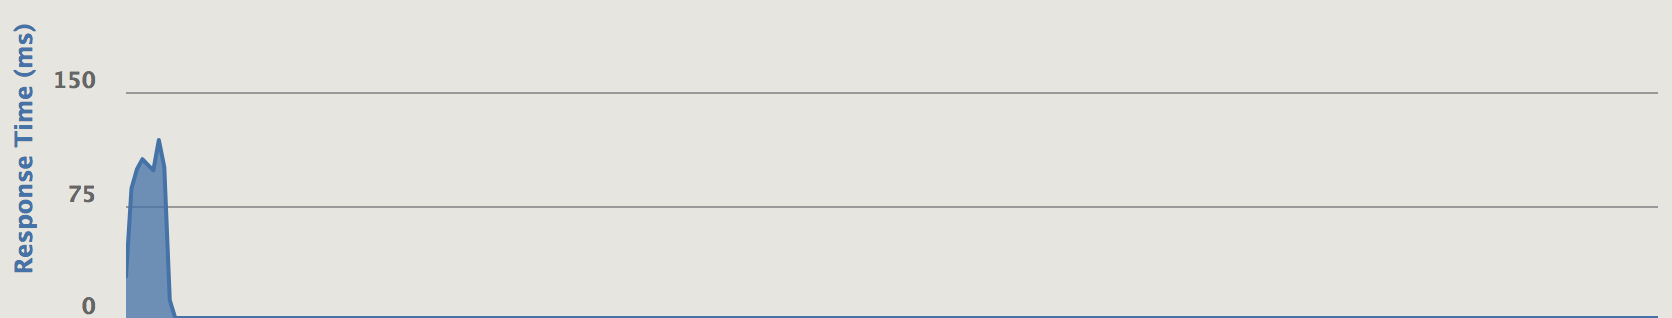
\includegraphics[width=108mm]{images/res-time}
\caption{经过优化的获取结构脑胞体响应时间随时间的变化,高响应时间的请求集中在开始时,后续的请求响应时间几乎为零}
\label{res-time}
\end{figure}

\subsection{使用 Redis 和负载均衡降低响应时间}
在优化获取结构脑胞体的响应时间的过程中使用了浏览器端的缓存进行优化,这启发我们使用服务器端的缓存来进一步优化。Redis 是一个支持网络、可基于内存亦可持久化的日志型、Key-Value 数据库\upcite{redis}。由于用户大概率修改编辑最新导入的数据,因此可以将近期的原始图像数据信息缓存在 Redis 之中,减少了请求数据库的次数,提升了整体性能。此外将数据库与网络服务器部署在不同的服务器上,降低了单台服务器的压力,大大提升了每秒响应请求的数量,使之可以支撑更多的用户同时访问。由于网络服务器的处理压力仍然较大,进一步将网络服务器的处理任务分散到两台服务器上,进一步降低了网络服务器的计算压力,优化过后的测试结果如图 \ref{opt} 所示,详细的测试分析在第四章论述。

\begin{figure}[!ht]
\centering
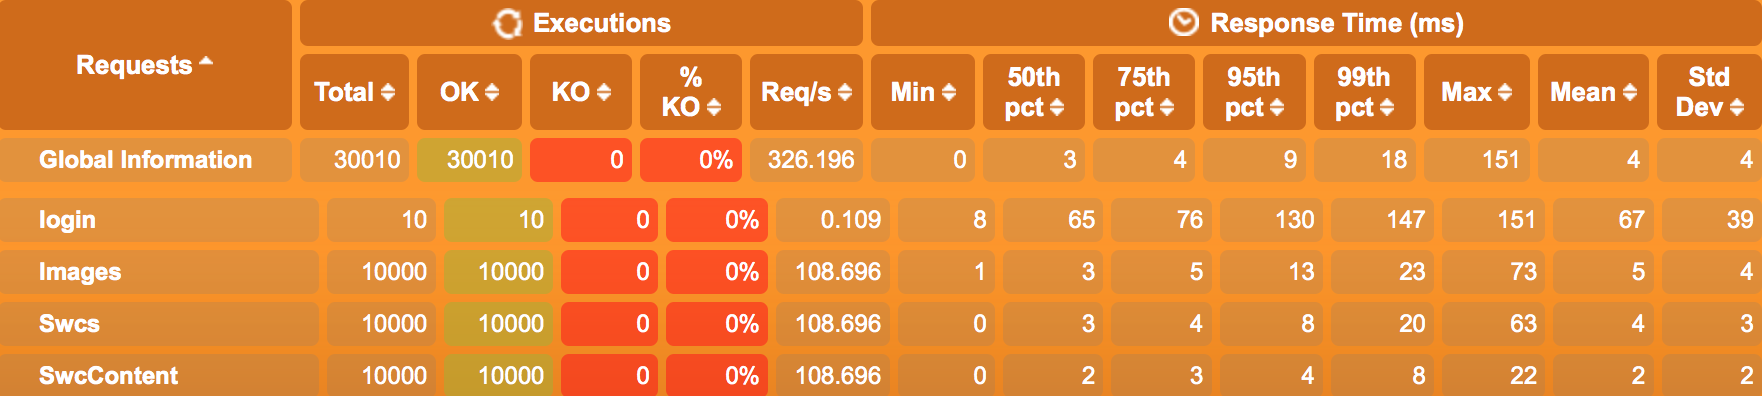
\includegraphics[width=108mm]{images/opt}
\caption{经过优化的整体响应时间报告,图中 Login 代表用户登录的请求, Images 代表获取用户原始图像列表相关 API 的响应时间,Swcs 代表用户对神经元结构进行操作的相关 API 的响应时间,SwcContent 代表用户获取结构脑胞体的响应时间。可以看出绝大多数响应时间都在 100 ms 一下,性能大大提升。}
\label{opt}
\end{figure}

\section{本章小结}
本章主要讨论了如何将用户的编辑操作转化成可以储存在数据库中的操作序列,描述了用户操作在三种不同层次上的抽象,根据实际需要选择不同层次的抽象,合理高效的储存了用户编辑操作,保证了结构脑胞体的有效性,并支持多用户操作合并,操作撤回等功能。讨论了用户信息数据库与神经信息数据库的实现细节,平台部署环境与方法,并根据性能测试报告进行了一系列的性能优化。

    \cleardoublepage
    \chapter{平台实际效果}
平台 UI 界面主要包含了用户信息管理与交互式神经元编辑两部分界面,使用了 Ant Design\upcite{antdesign} 作为设计规范和组件设计语言,three.js\upcite{threejs} 作为 3D 引擎实现交互式实时 3D 神经元编辑。本章主要展示了前端界面,并分析了平台实际性能。

\section{前端界面展示}
图 \ref{login} 展示了用户登录界面,图 \ref{register} 展示了用户注册界面,图中的“Hatu”是平台名称。

\begin{figure}[!ht]
\begin{minipage}[t]{0.5\linewidth} 
    \centering  
    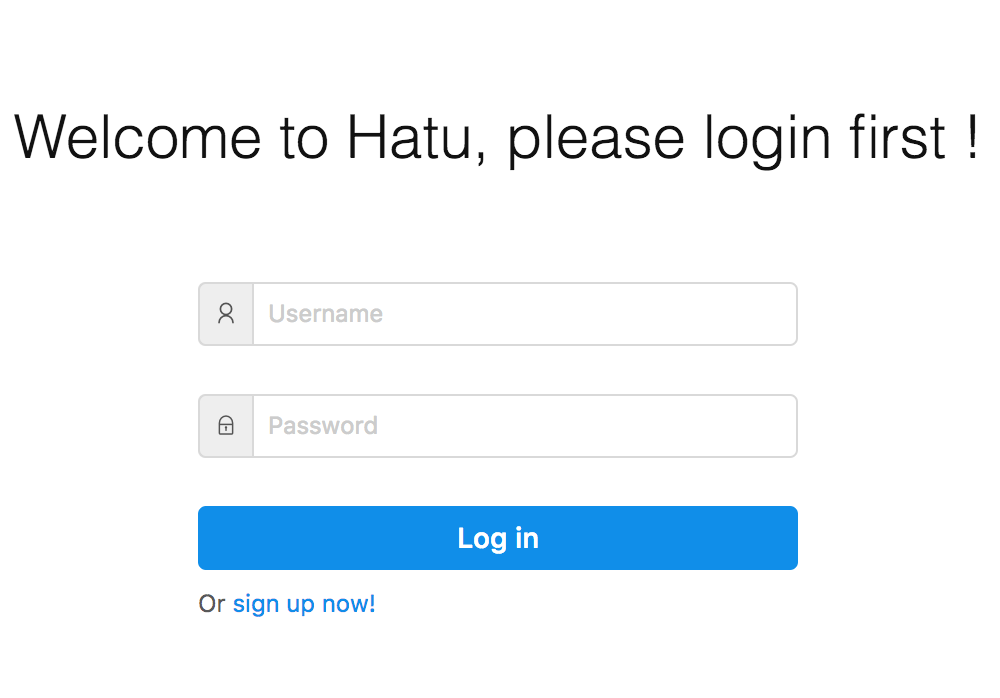
\includegraphics[width=7cm]{images/login}  
    \caption{用户登录界面}
    \label{login}  
    \end{minipage}  
    \begin{minipage}[t]{0.5\linewidth}
    \centering  
    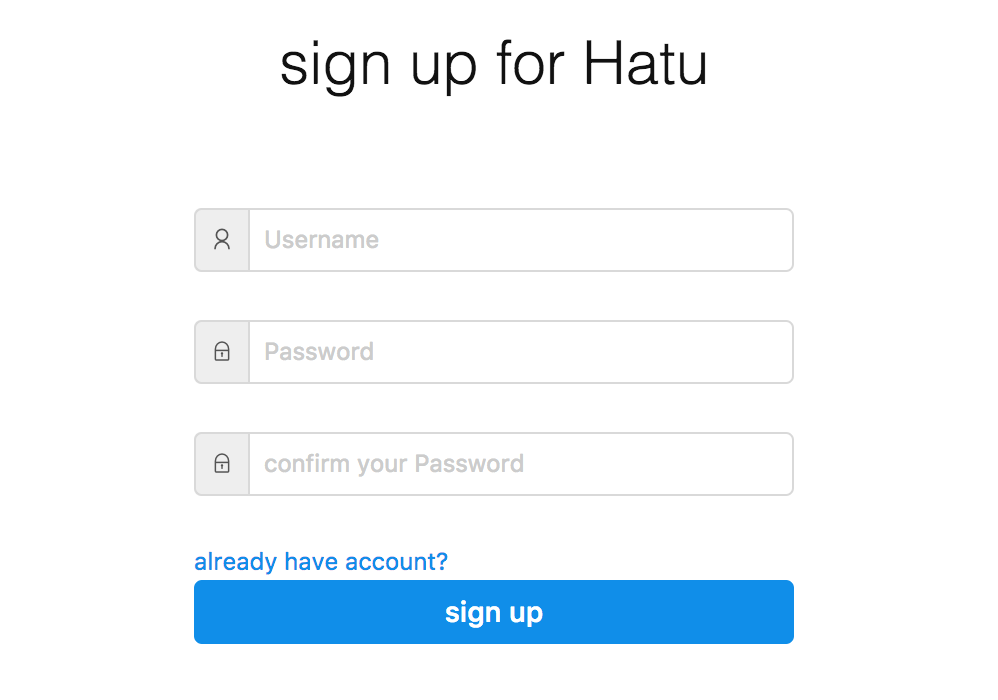
\includegraphics[width=7cm]{images/register}  
    \caption{用户注册界面}  
    \label{register}  
    \end{minipage}  
\end{figure}

\begin{figure}[!ht]
\begin{minipage}[t]{0.5\linewidth}
    \centering  
    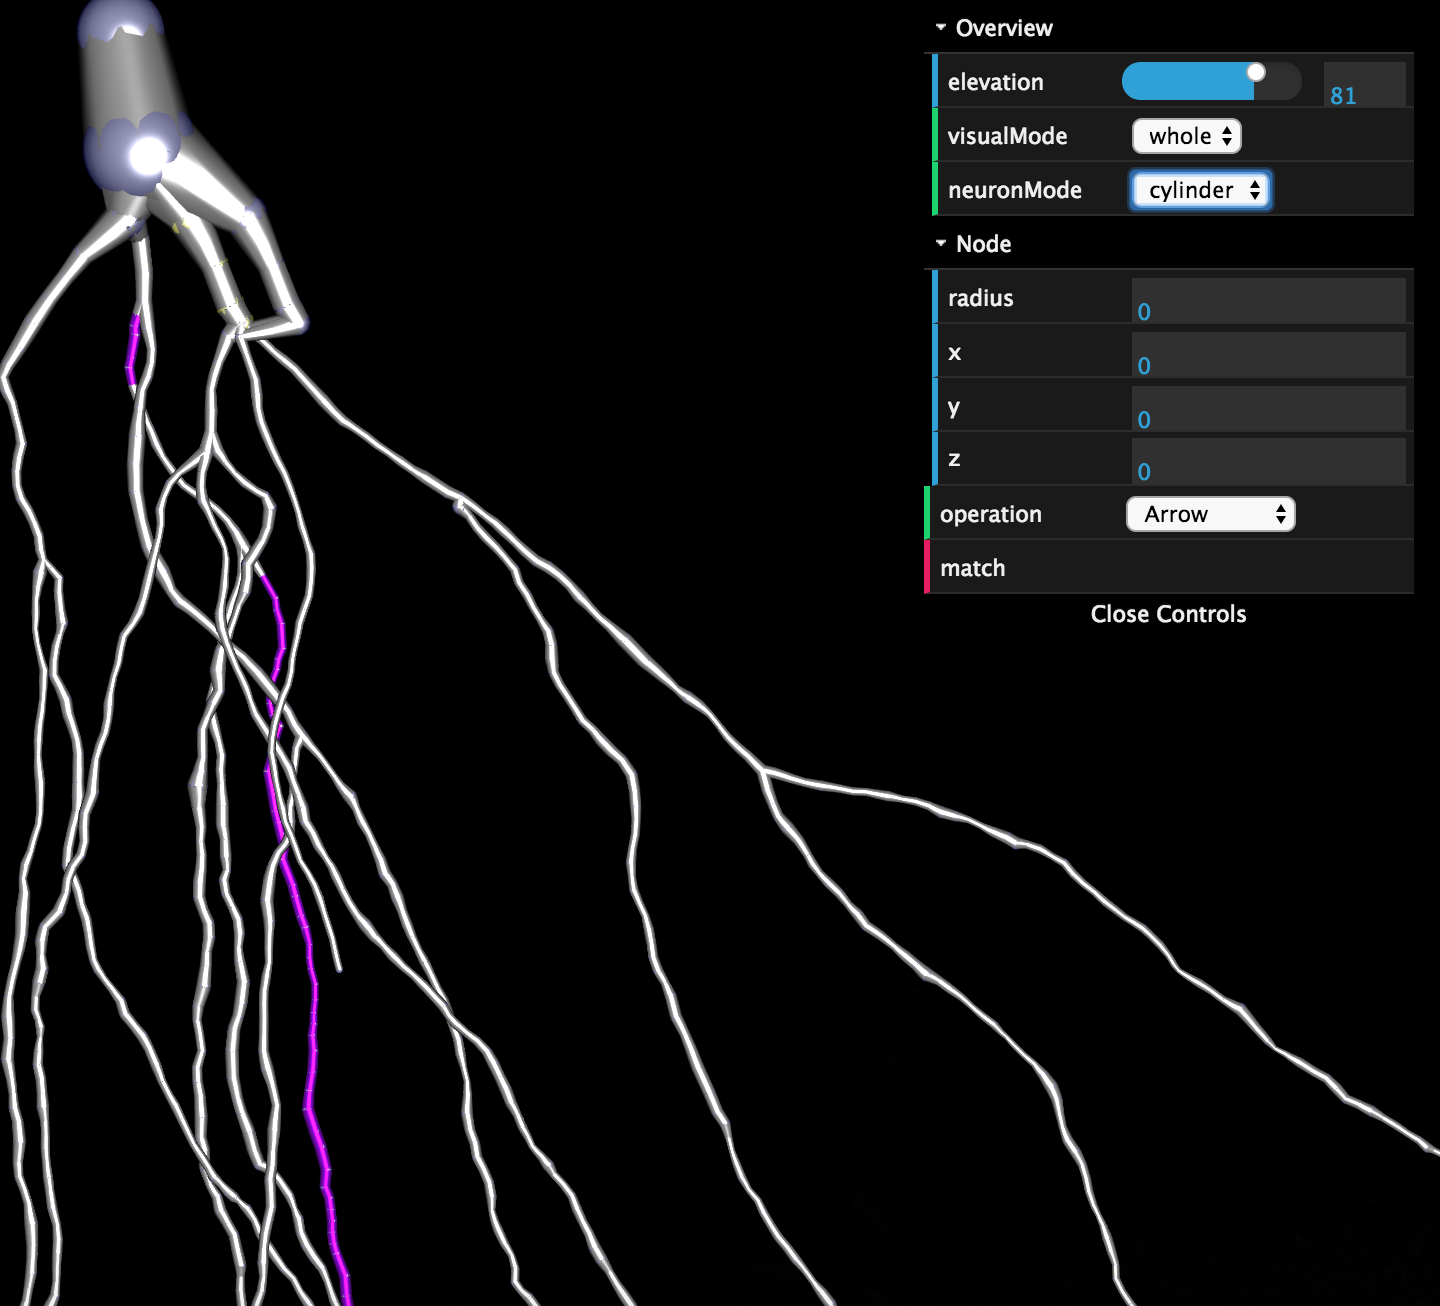
\includegraphics[width=7cm]{images/cylinder}  
    \caption{3D 柱状模式下交互式编辑界面}
    \label{cylinder}  
    \end{minipage}  
    \begin{minipage}[t]{0.5\linewidth} 
    \centering  
    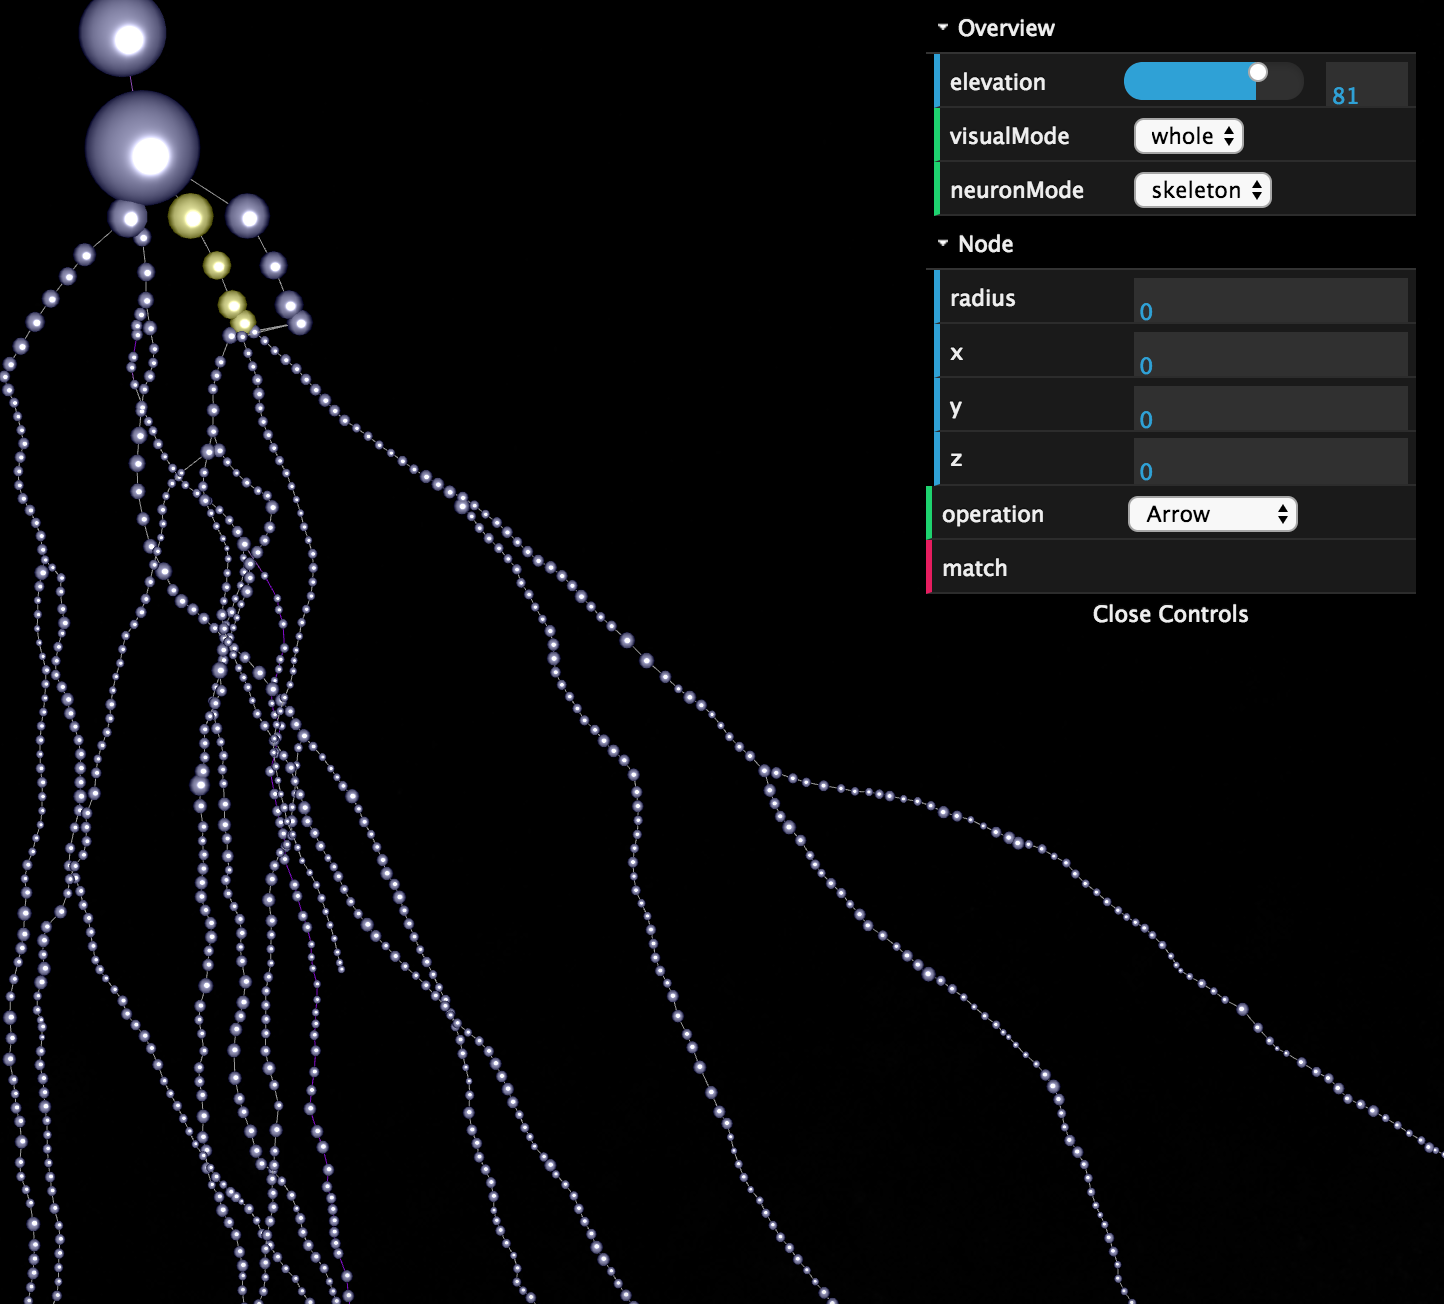
\includegraphics[width=7cm]{images/skeleton}  
    \caption{3D 骨架模式下交互式编辑界面}  
    \label{skeleton}  
\end{minipage} 
\begin{minipage}[t]{0.5\linewidth}
    \centering  
    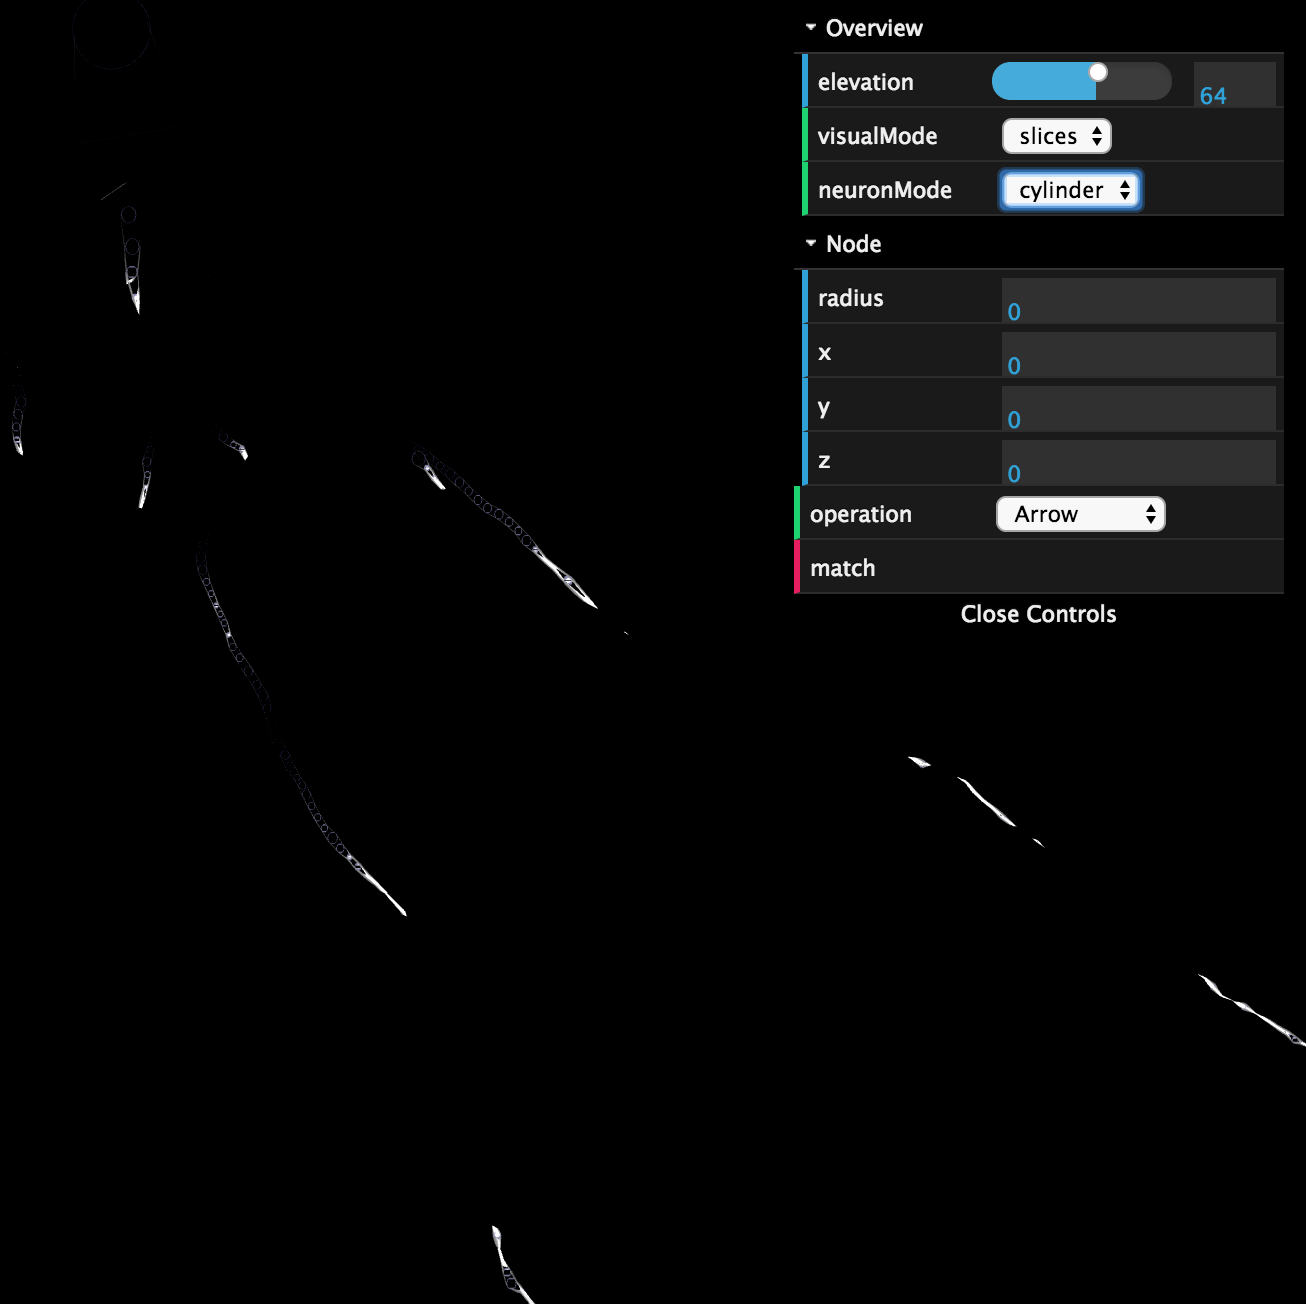
\includegraphics[width=7cm]{images/slice}  
    \caption{2D 切片模式下交互式编辑界面}
    \label{slice}  
\end{minipage}   
\end{figure}

\begin{figure}[!ht]
\begin{minipage}[t]{0.19\linewidth}
    \centering  
    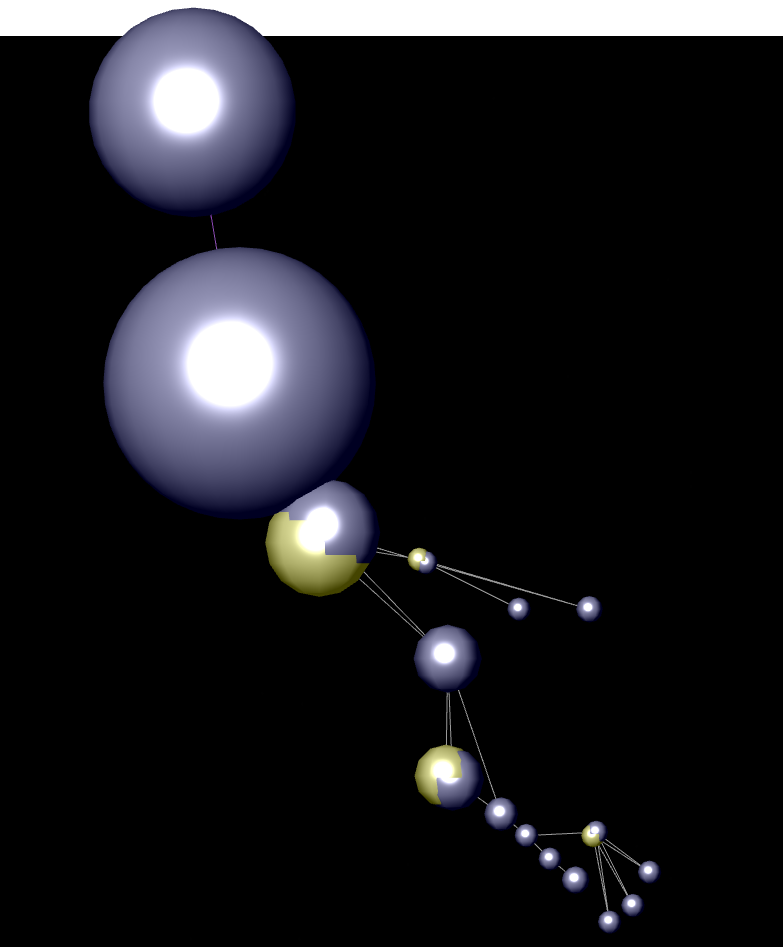
\includegraphics[width=2.8cm]{images/a0}   
\end{minipage}  
\begin{minipage}[t]{0.19\linewidth} 
    \centering  
    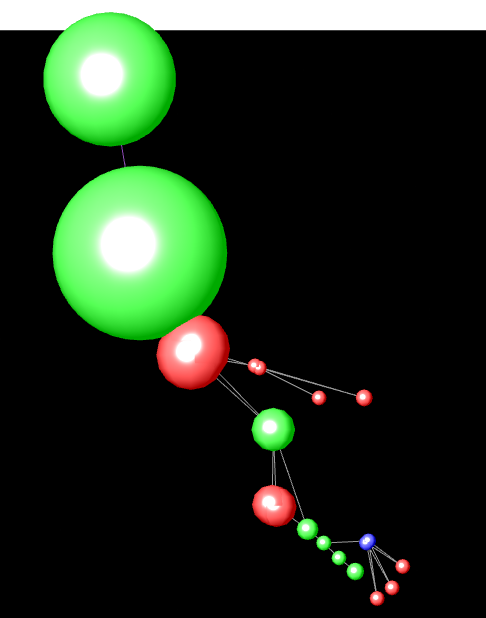
\includegraphics[width=2.8cm]{images/a1}  
\end{minipage} 
\begin{minipage}[t]{0.19\linewidth}
    \centering  
    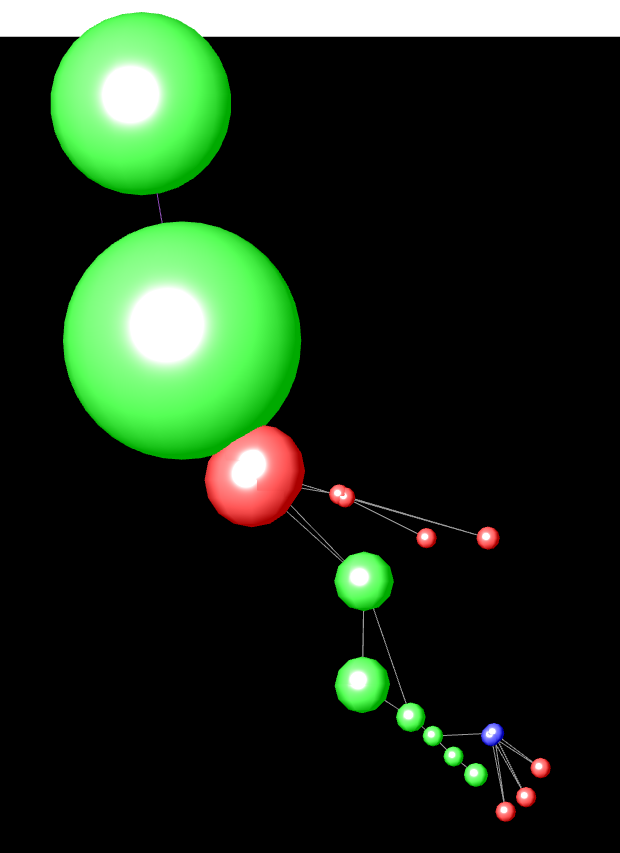
\includegraphics[width=2.8cm]{images/a2}    
\end{minipage}   
\begin{minipage}[t]{0.19\linewidth}
    \centering  
    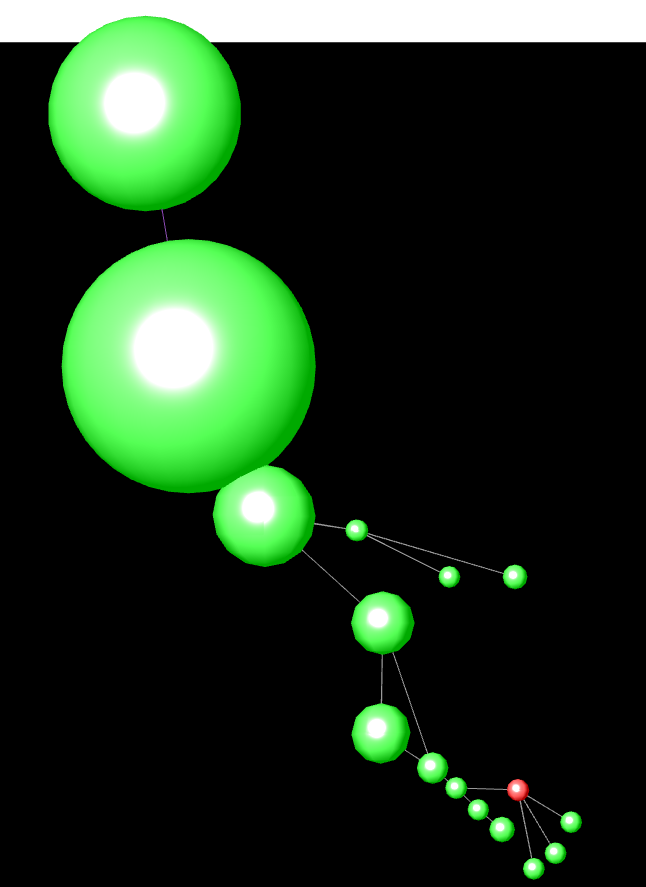
\includegraphics[width=2.8cm]{images/a3}   
\end{minipage}   
\begin{minipage}[t]{0.19\linewidth}
    \centering  
    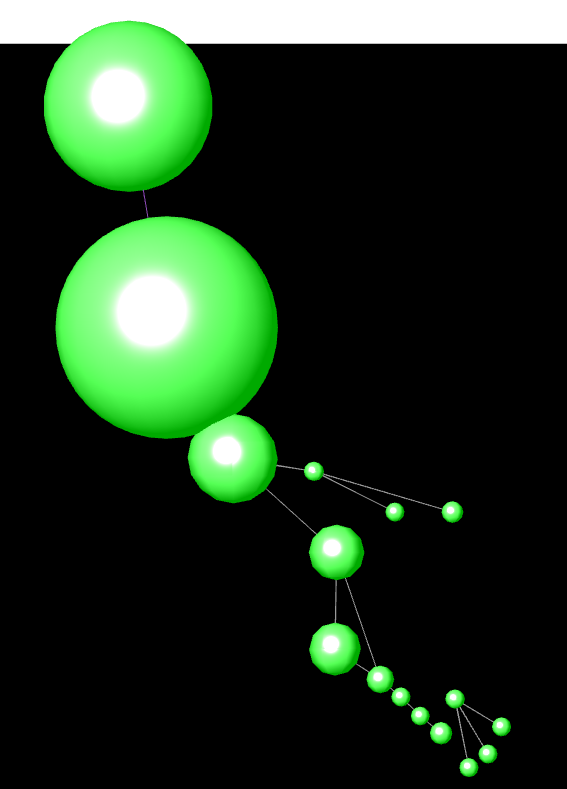
\includegraphics[width=2.8cm]{images/a4}   
\end{minipage} 
\caption{多用户协同编辑时结果合并的操作序列}
\label{merge}     
\end{figure}

图 \ref{cylinder} 展示了 3D 柱状模式下交互式编辑界面,图 \ref{skeleton} 展示了 3D 骨架模式下交互式编辑界面,图 \ref{slice} 展示了 2D 切片模式下交互式编辑界面。不同交互模式的适用场景不同。3D 模式适用于概览神经元整体结构,但是不适合精心调整,尤其不适合调整深度信息。2D 界面适合精细调整,可以和原始切片图像信息进行对比,保证调整的精确度,但是只能看到一个切片内的信息,难以查看神经元结构整体。神经科学家在使用时应根据具体的使用场景选取不同的模式。

图 \ref{cylinder} 与 图 \ref{skeleton} 展示 3D 模式下用不同颜色的球标明了团队中其他人员的修改,当前编辑人员可以决定保存团队中其他人员的修改或者进一步进行修改,系统会自动根据两者的修改内容进行合并,这部分算法由前端可视化完成,本文不详细论述。在编辑完成之后可以选择将编辑成果分享给其他神经科学家,使得团队协作变得更加简洁。

\section{前端请求实际性能}
\subsection{静态文件请求}
经过 webpack 打包过后只有两个 js 文件与一个 css 文件。两个 js 文件中一个是前端程序员编写的代码另一个是依赖的第三方代码。图 \ref{file-nocache} 示了静态资源文件的大小与第一次获取的时间。由于可视化任务较为复杂,即使在压缩过后仍有 2MB 左右的大小,在第一次未缓存的状况下有 4s 的加载时间,用户能明显的感受到加载时间。图 \ref{file-cache} 展示了缓存后的加载时间,此时只需要一百毫秒的时间即可完成加载,也就是说用户在后续的访问中不会感受到延迟。 

\begin{figure}[!ht]
\centering
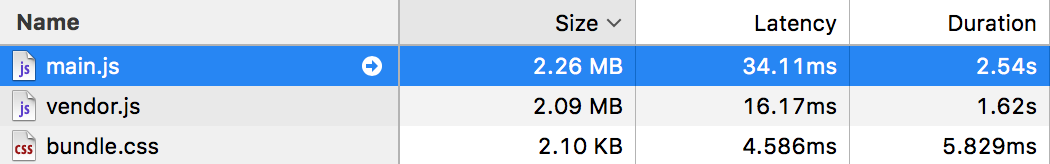
\includegraphics[width=148mm]{images/file-nocache}
\caption{静态资源文件大小与未缓存时所需的加载时间}
\label{file-nocache}
\end{figure}

\begin{figure}[!ht]
\centering
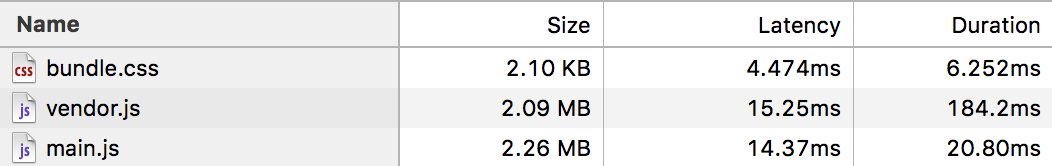
\includegraphics[width=148mm]{images/file-cache}
\caption{静态资源文件大小与缓存后所需的加载时间}
\label{file-cache}
\end{figure}

\subsection{登录与注册请求}
图 \ref{login-res} 展示了用户登录请求响应时间,图 \ref{signup-res} 展示了用户注册响应时间。从图中可以看出登录请求用时 24.40 ms,注册请求用时 183.37ms,属于用户可以接受的范围内。注册请求较登录请求响应时间更长是由于注册新用户是需要初始化神经信息数据库,这需要消耗一定的时间。

\begin{figure}[!ht]
\centering
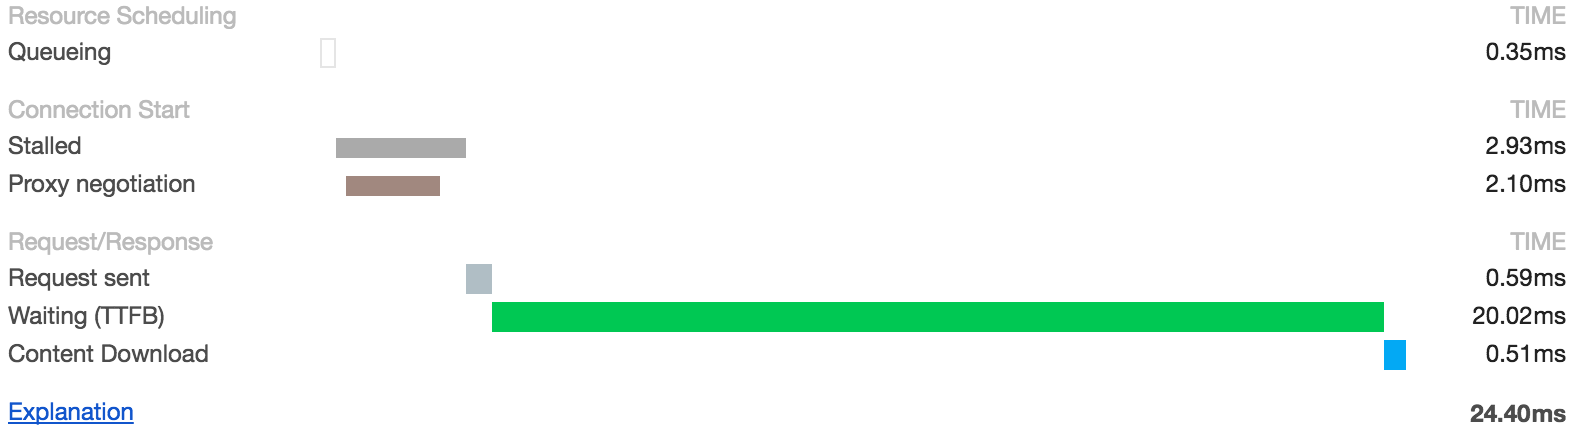
\includegraphics[width=128mm]{images/login-res}
\caption{用户登录请求响应时间}
\label{login-res}
\end{figure}

\begin{figure}[!ht]
\centering
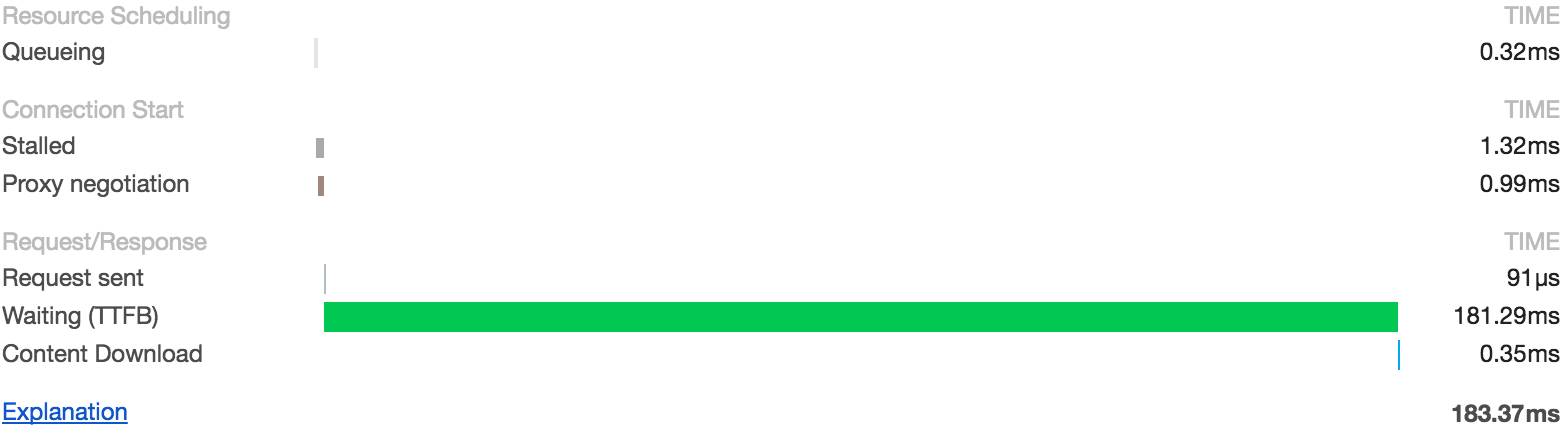
\includegraphics[width=128mm]{images/signup-res}
\caption{用户注册请求响应时间}
\label{signup-res}
\end{figure}

\subsection{动态请求}
图 \ref{dy-res} 展示了动态请求的大小,数据和\ref{chap3}中测试数据一致,最长响应时间在 100ms 左右,用户不会感受到明显的卡顿。值得注意的是两个 slice15 请求和两个 slice15\_L11.swc 请求。两次请求的响应时间一个从 89.37ms 下降到 37.95ms,另一个从 109.0ms 下降到 13.50ms 再一次说明了使用缓存对性能的巨大提升。

\begin{figure}[!ht]
\centering
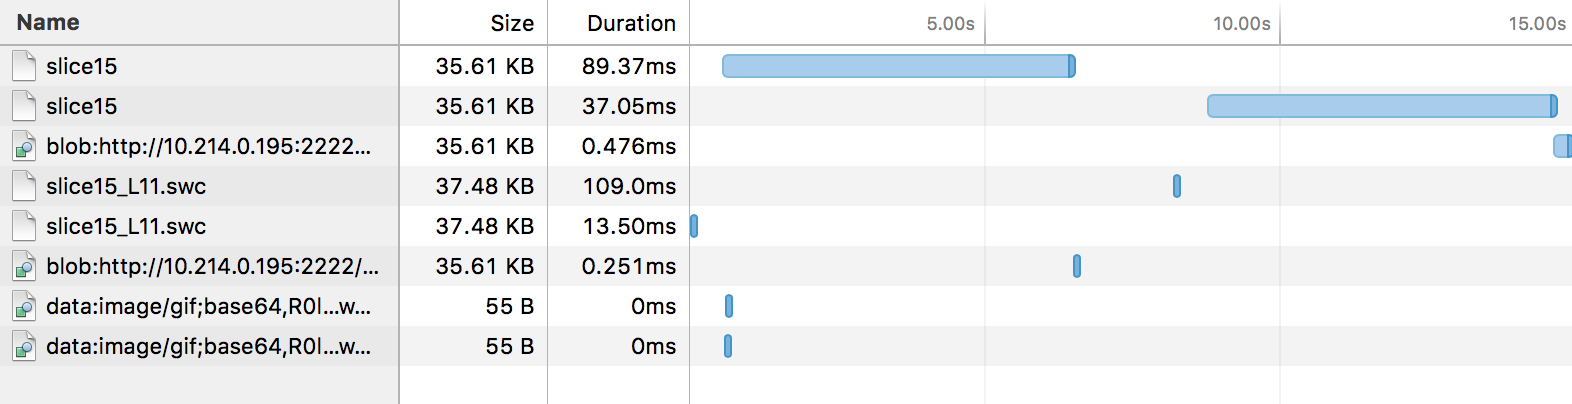
\includegraphics[width=148mm]{images/dy-res}
\caption{动态请求大小与请求响应时间}
\label{dy-res}
\end{figure}

\section{本章小结}
本章展示了用户信息管理与交互式神经元编辑两部分前端界面,并详细分析了静态文件请求,登录与注册请求与动态请求三种前端请求,与\ref{chap3}中压力测试的结果进行验证。绝大多数的请求均可在毫秒级别响应,保证了前端可视化与编辑操作的流畅。目前存在的问题是两个 js 文件过大,用户在第一次访问时能感受到明显的加载时间。需要进一步研究相关技术,压缩 js 文件的大小。
    \cleardoublepage
    \renewcommand{\thechapter}{}
    \bibliographystyle{data/gbt7714-2005}
\bibliography{data/bibliography}
\addcontentsline{toc}{chapter}{\bibname}

    \cleardoublepage
    \chapter*{致谢}
\addcontentsline{toc}{chapter}{致谢}
\markright{致谢}

待写。

    \cleardoublepage
  }

  {
    \backmatter

    \pagestyle{empty}

    {
  \setlength{\parindent}{0em}
  \linespread{1}

  \vspace*{-2.2em}

  {
    \centering
    \songti\erhao\bfseries
    本科生毕业论文(设计)任务书 \par
  }

  \vspace{2.1em}

  {
    \songti\xiaosi\bfseries
    一、 \; 题目 \; \underline{\makebox{\zjutitlec}}

    \vspace{1.1em}

    二、 \; 指导教师对毕业论文(设计)的进度安排及任务要求

    \vspace{15.5em}

    \hfill 起讫日期 \hspace{2em} 年 \hspace{1em} 月 \hspace{1em} 日 \; 至 \hspace{2em} 年 \hspace{1em} 月 \hspace{1em} 日

    \vspace{1.3em}

    \hfill 指导教师(签名) \; \underline{\hspace{4em}} \; 职称 \; \underline{\hspace{4em}}

    \vspace{2.35em}

    三、 \; 学院审核意见

    \vspace{13.95em}

    \hfill 负责人(签名) \; \underline{\hspace{4em}}

    \vspace{1.3em}

    \hfill \hspace{2em} 年 \hspace{1em} 月 \hspace{1em} 日 \par
  }
}

    {
  \setlength{\parindent}{0em}
  \linespread{1}

  \vspace*{-2.1em}

  {
    \centering
    \songti\xiaoer\bfseries
    毕~~业~~论~~文~~(设~~计)~~考~~核 \par
  }

  \vspace{1.1em}

  {
    \songti\sihao\bfseries
    一、\; 指导教师对毕业论文(设计)的评语 \par
  }
    ~~~~~~针对大规模神经元重建任务的实际需求,论文设计并实现了支持1000个用户操作的服务器版本,进行了系统级的优化,并进行了服务器运行参数的广泛测试。进一步的工作将在硬件系统到位后,由用户进行实际操作测试,以推进系统的进一步真正的实用化过程。毕业设计推进顺利,完成了预定的目标。

  \vspace{8em}

  {
    \songti\xiaosi\bfseries
    \hfill 指导教师(签名) \; \underline{\hspace{5em}}

    \vspace{0.1em}

    \hfill \hspace{2em} 年 \hspace{1em} 月 \hspace{1em} 日 \par
  }

  \vspace{0.7em}

  {
    \songti\sihao\bfseries
    二、 \; 答辩小组对毕业论文(设计)的答辩评语及总评成绩:
  }

  \vspace{14.7em}

  {
    \renewcommand{\arraystretch}{1.5}
    \songti\xiaosi\bfseries
    \hfill \begin{tabular}{|c|m{4.1em}|m{4.1em}|m{4.1em}|m{9.1em}|c|}
      \hline
      成绩比例 & {\centering 开题报告 \\ 占(20\%)} & {\centering 外文翻译 \\ 占(10\%)} & {\centering 文献综述 \\ 占(10\%) } & {\centering 毕业论文(设计) \\ 质量及答辩占(60\%)} & 总成绩 \\
      \hline
      分值 & & & & & \\
      \hline
    \end{tabular} \par
  }

  \vspace{2em}

  {
    \songti\xiaosi\bfseries
    \hfill 答辩小组负责人(签名) \; \underline{\hspace{5em}}

    \vspace{0.1em}

    \hfill \hspace{2em} 年 \hspace{1em} 月 \hspace{1em} 日 \par
  }
}

  }

\end{document}
